\documentclass[fr]{../../../eplnotes}
\usepackage{../../../eplunits}
\usepackage{pgfplots}
\pgfplotsset{compat=newest}
\usepgfplotslibrary{fillbetween}
\usetikzlibrary{external}
\usetikzlibrary{patterns}
\usetikzlibrary{arrows}
\usetikzlibrary{calc}
\tikzexternalize[prefix=figures/]
\numberwithin{equation}{section}

\hypertitle{thermo-MECA1855}{5}{MECA}{1855}
{Adrien Couplet}%\and Marie-Pierre van Oldeneel}
{Miltiadis Papalexandris et Yann Bartosiewicz}[
\paragraph{Remarque} Ce document a pour objectif de rassembler et de répondre en détails aux questions de théorie du cours en vue
de l’examen. Celles-ci ont soit été fournies par M. Papalexandris sur Moodle, soit proviennent d'anciens examens. Le document suppose une compréhension préalable de la matière et ne fait office ni de synthèse, ni de syllabus.]

\section{Questions sur le chapitre ``Introduction et rappels''}
\subsection{Est-ce que la chaleur échangée entre un système et son extérieur est une variable d'état du système. Justifiez votre réponse.}
Une \textbf{variable d'état} caractérise un état et non une évolution entre deux états. La chaleur échangée $Q$ entre un système et son extérieur décrit le passage d'un état à un autre et ne peux pas être mesurée instantanément. Les variables d'état d'un système thermodynamique sont par exemple la pression $p$, le volume $V$ ou encore la température $T$. 

\subsection{Donnez la définition d'un processus \textit{adiabatique}. Donner un exemple d'un processus adiabatique réversible ainsi qu'un exemple d'un processus adiabatique irréversible.}
Une transformation est dite \textbf{adiabatique} si elle est effectué sans échange de chaleur ($Q = 0$). Cela n'implique pas pour autant que la température du système reste constante. La variation d'énergie mécanique est le seul échange avec l'extérieur du système qui modifie alors les variables d'états ($T$, $V$ et $p$).

Le concept de \textbf{réversibilité} est idéal. L'expression énergétique du second principe de la thermodynamique, aussi appelé principe d'évolution, s'écrit 
\begin{equation} Q + W_f = \int_1^2T dS \end{equation}
où $dS$ est la différentielle de la fonction d'état entropie et $W_f$ le terme dissipatif. Dans la réalité ce terme ne sera jamais nul. 
\begin{itemize}
	\item Un processus \textbf{réversible} est un processus où $W_f = 0$. Un processus adiabatique réversible est donc aussi isentropique car $\delta Q/T = dS = 0$. Un exemple d'un tel processus se trouve dans le cycle de Carnot qui comprend une détente ainsi qu'une compression adiabatique réversible. Il est à noter que le cycle de Carnot est un cycle théorique.
	\item Un processus \textbf{irréversible} est un processus où $W_f \neq 0$. On retrouve une détente adiabatique irréversible dans les cycle frigorifique. 
\end{itemize}

\subsection{Donnez la définition mathématique ainsi que la signification physique des chaleurs massiques $c_p$ et $c_v$.}
La capacité thermique massique $c$ correspond à la quantité d'énergie à apporter par échange thermique pour élever d''un kelvin la température de l'unité de masse d'une substance. C'est donc une grandeur intensive exprimé en joules par kilogramme-kelvin \si{\joule\per\kelvin\per\kilo\gram}. Si on note $U$ l'énergie interne, $H$ l'enthalpie et $m$ la masse d'un corps on a les capacités thermiques massiques :
\begin{itemize}
	\item à pression constante \begin{equation} c_p = \frac{1}{m}\left(\frac{\partial H}{\partial T}\right)_p \end{equation}
	\item à volume constant \begin{equation} c_v = \frac{1}{m}\left(\frac{\partial U}{\partial T}\right)_V \end{equation}
\end{itemize}

\subsection{Donnez la définition de l'enthalpie libre $F$ de Helmholtz ainsi que de l'enthalpie libre $G$ de Gibbs. Écriver l'équation de Gibbs sous la forme de différentielle de $F$ ainsi que de $G$.}
\paragraph{L'énergie libre $F$ de Helmholtz} est une fonction d'état extensive dont la variation permet d'obtenir le travail utile susceptible d'être fourni par un système fermé, à température constante, au cours d'une transformation réversible. 
Considérons un système thermodynamique (fermé) évoluant d'un état 1 à un état 2, transformation que l'on suppose totalement réversible ($W_f = 0$) et à température constante $T$. Le premier principe de la thermodynamique s'exprime par :
\begin{equation} \Delta U + \Delta K + g\Delta z = Q + \underline{W_e} \end{equation}
où $\Delta U$ désigne la variation de l'énergie interne, $\Delta K$ la variation de l'énergie cinétique, $g\Delta z$ la variation de l'énergie potentielle, $Q$ l'échange de chaleur et $\underline{W_e}$ le travail des forces extérieures. On introduit $W = -W_e$ qui correspond au travail récupérable par le milieu extérieur et on suppose $\Delta K = g\Delta z = 0$. On obtient alors
\begin{equation} W = Q - \Delta U \label{eq:Q1ePrincipe}\end{equation}
Le 2\ieme principe de la thermodynamique s'exprime par:
\begin{equation} \Delta S = \frac{Q}{T} + W_f \qquad\Leftrightarrow\qquad Q = T\Delta S - TW_f \label{eq:Q2ePrincipe}\end{equation}
où $\Delta S$ est la variation d'entropie du système. Si on remplace \ref{eq:Q2ePrincipe} dans \ref{eq:Q1ePrincipe}, nous trouvons
\begin{equation} W = T\Delta S - TW_f - \Delta U = T(S_2 - S_1) - TW_f + U_1 - U_2 \end{equation}
Il est évident, d'après la relation obtenue, que $W$ sera maximum si la transformation est totalement réversible ($W_f = 0$) :
\begin{equation} W_\text{max} = (U_1 - TS_1)-(U_2-TS_2)\end{equation}
On définit alors 
\begin{equation} F = U - TS \end{equation} 
Ce qui nous donne au final 
\begin{equation} W_\text{max} = -\Delta F \qquad\text{où}\qquad \underbrace{\Delta F}_\text{travail utile} = \underbrace{\Delta U}_\text{énergie totale} - \underbrace{T\Delta S}_\text{énergie inutilisable}\end{equation}

\paragraph{Forme différentielle de $F$}
\begin{equation} \left.\begin{array}{ll} dF &= d(U-TS) = dU - TdS - SdT \\ dU &= -pdV + TdS \end{array}\right\} \Rightarrow dF = -pdV - SdT\end{equation}

\paragraph{L'enthalpie libre $G$ de Gibbs} est une fonction d'état extensive dont la variation permet d'obtenir l'enthalpie utile susceptible d'être fournie par un système fermé, à température et à pression constante, au cours d'une transformation réversible. On considère le même système que précedemment avec la condition supplémentaire que la pression est constante. Par la définition de l'enthalpie :
\begin{equation} H \triangleq U + pV\end{equation}
De la même manière que pour l'énergie libre de Helmholtz, on trouve :
\begin{equation} W = Q - \Delta H \label{H1ePrincipe}\end{equation}
où $W$ correspond à nouveau au travail récupérable par le milieu extérieur. Si on remplace \ref{eq:Q2ePrincipe} dans \ref{H1ePrincipe} et qu'on prend on compte le fait que le processus est réversible, on obtient :
\begin{equation} W_\text{max} = (H_1 - TS_1) - (H_2 - TS_2) \end{equation}
On définit alors
\begin{equation} G = H - TS \end{equation}

\paragraph{Forme différentielle de G}
\begin{equation} \left.\begin{array}{ll} dG &= d(H-TS) = dH - TdS - SdT \\ dH &= Vdp + TdS \end{array}\right\} \Rightarrow dG = Vdp - SdT \label{eq:gibbs-duhem}\end{equation}

\subsection{Dérivez l'équation $\alpha = p\beta K$.}
Les variables d'état $p$, $v$ et $T$ d'un fluide sont liées par l'équation d'état, que l'on peut écrire sous forme du système différentiel :
\begin{equation}\begin{pmatrix} dp \\ dv \\ dT \end{pmatrix} = \begin{pmatrix} 0 & \left(\frac{\partial p}{\partial v}\right)_T & \left(\frac{\partial p}{\partial T}\right)_v \\ \left(\frac{\partial v}{\partial p}\right)_T & 0 & \left(\frac{\partial v}{\partial T}\right)_p \\ \left(\frac{\partial T}{\partial p}\right)_v & \left(\frac{\partial T}{\partial v}\right)_p & 0 \end{pmatrix}\begin{pmatrix} dp \\ dv \\ dT \label{eq:matetat}\end{pmatrix}\end{equation}
On définit les coefficients suivants :
\begin{itemize}
	\item le coefficient de dilatation isobare $\alpha \triangleq \frac{1}{v}\left(\frac{\partial v}{\partial T}\right)_p$
	\item le coefficient de dilatation isochore $\beta \triangleq \frac{1}{p}\left(\frac{\partial p}{\partial T}\right)_v$
	\item le coefficient de compressibilité isotherme $K \triangleq -\frac{1}{v}\left(\frac{\partial v}{\partial p}\right)_T$
\end{itemize}
Le système \ref{eq:matetat} peut se réécrire sous la forme :
\begin{equation}\begin{pmatrix} dp \\ dv \\ dT \end{pmatrix} = \begin{pmatrix} 0 & -\frac{1}{Kv} & \beta p \\ -Kv & 0 & \alpha v \\ \frac{1}{\beta p} & \frac{1}{\alpha v} & 0 \end{pmatrix}\begin{pmatrix} dp \\ dv \\ dT \end{pmatrix} \label{eq:fe_matrix}\end{equation}
On trouve l'équation recherchée à l'aide des variations de deux des trois variables d'état: 
\begin{equation} dp = -\frac{1}{Kv}dv + \beta p dT \label{eq:dp}\end{equation}
\begin{equation} dv = -Kv dp +  \alpha v dT \label{eq:dv}\end{equation}
En remplacant le terme $dv$ dans l'équation \ref{eq:dp} par l'équation \ref{eq:dv} on obtient :
\begin{equation} dp = dp - \frac{\alpha}{K}dT + \beta p dT \qquad\Rightarrow\qquad \alpha = p\beta K\end{equation}
Cette équation nous permet de conclure que l'équation d'état d'une substance est déterminée par la connaissance de deux des trois coefficients caractéristiques $\alpha$, $\beta$ ou $K$.

\subsection{Démontrez que les expressions \ref{eq:q6_1} sont valables pour toutes les espèces.}
\begin{equation} \left(\frac{\partial T}{\partial p}\right)_S = \left(\frac{\partial v}{\partial S}\right)_p, \qquad \left(\frac{\partial S}{\partial p}\right)_T = - \left(\frac{\partial v}{\partial T}\right)_p \label{eq:q6_1}\end{equation}
Toutes les fonctions d'état peuvent être exprimées en fonction de deux des trois variables d'état $p$, $v$ et $T$. Il en va de même pour l'entropie pour laquelle le système différentiel s'écrit :
\begin{equation}\begin{pmatrix}TdS\\TdS\\TdS\end{pmatrix} = \begin{pmatrix}0 & l_T & c_v \\ h_T & 0 & c_p \\ h_v & l_p & 0\end{pmatrix}\begin{pmatrix}dp\\dv\\dT\end{pmatrix} \end{equation}
On introduit ainsi quatre coefficients calorifiques $l_T$, $h_T$, $h_v$ et $l_p$ qui peuvent s'exprimer en fonction des coefficients calorifiques $c_p$ et $c_v$, et des coefficients de dilatation $\alpha$ et $\beta$ :
\begin{equation} h_v = \frac{c_v}{\beta p}, \qquad l_p = \frac{c_p}{\alpha v}, \qquad h_T = \frac{c_v-c_p}{\beta p}, \qquad l_T = \frac{c_p-c_v}{\alpha v}.\end{equation}
La substitution des expressions dans le système différentiel fournit la matrice $S'$ des dérivées partielles de l'entropie :
\begin{equation} S' = \begin{pmatrix} 0 & \frac{c_p-c_v}{\alpha vT} & \frac{c_v}{T} \\ \frac{c_v-c_p}{\beta pT} & 0 & \frac{c_p}{T} \\ \frac{c_v}{\beta pT} & \frac{c_p}{\alpha vT} & 0 \end{pmatrix} \end{equation}
Si on prend la deuxième ligne de ce système, on a :
\begin{equation} dS = \frac{c_v-c_p}{\beta pT}dp + \frac{c_p}{T}dT \qquad \Leftrightarrow \qquad \left(\frac{\partial T}{\partial p}\right)_S = \frac{c_p-c_v}{c_p\beta p} \end{equation}
Si on prend la troisième ligne de ce système, on a :
\begin{equation} dS = \frac{c_v}{\beta pT}dp + \frac{c_p}{\alpha vT}dv \qquad \Leftrightarrow \qquad \left(\frac{\partial v}{\partial S}\right)_p = \frac{\alpha vT}{c_p} \end{equation}
De la matrice \ref{eq:fe_matrix} on a :
\begin{equation} dv = -Kv dp + \alpha v dT \qquad \Leftrightarrow \qquad \left(\frac{\partial v}{\partial T}\right)_p = \alpha v \end{equation}
Avec la relation $c_p-c_v = \alpha\beta pvT$, on trouve finalement :
\begin{equation} \left(\frac{\partial T}{\partial p}\right)_S = \frac{c_p-c_v}{c_p\beta p} = \frac{\alpha vT}{c_p} = \left(\frac{\partial v}{\partial S}\right)_p \end{equation}
\begin{equation} \left(\frac{\partial S}{\partial p}\right)_T = \frac{c_v-c_p}{\beta pT} = \alpha v = \left(\frac{\partial v}{\partial T}\right)_p \end{equation}

\subsection{Dérivez l'équation $c_p-c_v = \alpha\beta pvT$.\label{q:1_7}}
On part des équations de Gibbs (énergie libre de Helmholtz et enthalpie libre de Gibbs) :
\begin{equation} \begin{cases} F &= U-TS \\ G &= H-TS \end{cases} \qquad \Rightarrow \qquad \begin{cases} dF &= -pdv - SdT \\ dG &= vdp - SdT \end{cases} \end{equation}
Ces différentielles correspondent aux expressions des dérivées partielles suivantes :
\begin{equation} \left(\frac{\partial F}{\partial v}\right)_T = -p \qquad \left(\frac{\partial F}{\partial T}\right)_v = -S \qquad \left(\frac{\partial G}{\partial p}\right)_T = v \qquad \left(\frac{\partial G}{\partial T}\right)_p = -S \end{equation}
Soit un potentiel thermodynamique $\Phi$ étant présumé au moins deux fois dérivable par rapport à chacune de ses variables. Le \textbf{théorème de Schwarz}\footnote{\url{https://fr.wikipedia.org/wiki/Th\%C3\%A9or\%C3\%A8me_de_Schwarz}} implique que pour tout couple de variable $x_i$ et $x_j$ :
\begin{equation} \left(\frac{\partial}{\partial x_i}\left(\frac{\partial \Phi}{\partial x_j}\right)_{x_{k\neq j}}\right)_{x_{k\neq i}} = \left(\frac{\partial}{\partial x_j}\left(\frac{\partial \Phi}{\partial x_i}\right)_{x_{k\neq i}}\right)_{x_{k\neq j}} \end{equation}
Si on applique le théorème de Schwarz, on obtient :
\begin{equation} \frac{\partial^2F}{\partial T\partial v} = -\left(\frac{\partial p}{\partial T}\right)_v = -\beta p , \qquad \frac{\partial^2F}{\partial v\partial T} = -\left(\frac{\partial S}{\partial v}\right)_T = -\frac{c_p-c_v}{\alpha vT} \end{equation}
\begin{equation} \frac{\partial^2G}{\partial T\partial p} = \left(\frac{\partial v}{\partial T}\right)_p = \alpha v , \qquad \frac{\partial^2G}{\partial p\partial T} = -\left(\frac{\partial S}{\partial p}\right)_T = -\frac{c_v-c_p}{\beta vT} \end{equation}
Ce qui entraîne la propriété liant entre elles les chaleurs massique $c_p$ et $c_v$ :
\begin{equation} c_p-c_v = \alpha\beta pvT \label{eq:relation_chaleur}\end{equation}

\subsection{Dérivez l'équation \ref{eq:q8}}
\begin{equation} l_T = \frac{c_p-c_v}{\alpha v} \label{eq:q8}\end{equation}
Toutes les fonctions d'état peuvent être exprimées en fonction de deux des trois variables d'état $p$, $v$ et $T$. Il en va de même pour l'entropie pour laquelle le système différentiel s'écrit :
\begin{equation}\begin{pmatrix}TdS\\TdS\\TdS\end{pmatrix} = \begin{pmatrix}0 & l_T & c_v \\ h_T & 0 & c_p \\ h_v & l_p & 0\end{pmatrix}\begin{pmatrix}dp\\dv\\dT\end{pmatrix} \end{equation}
En remplacant la variation de température $dT$ dans la première et seconde équations du système par 
\begin{equation} dT = \frac{1}{\beta p}dp + \frac{1}{\alpha v}dv \end{equation}
on obtient :
\begin{equation}\begin{pmatrix}TdS\\TdS\\TdS\end{pmatrix} = \begin{pmatrix}\frac{c_v}{\beta p} & l_T + \frac{c_v}{\alpha v} & 0\\ h_T + \frac{c_p}{\beta p} & \frac{c_p}{\alpha v} & 0 \\ h_v & l_p & 0\end{pmatrix}\begin{pmatrix}dp\\dv\\dT\end{pmatrix} \end{equation}
L'identification des trois équations de ce système permet d'exprimer les quatres nouveaux coefficients calorifiques en fonction des seuls coefficients calorifiques $c_p$ et $c_v$, et des coefficients de dilatation $\alpha$ et $\beta$ :
\begin{equation} h_v = \frac{c_v}{\beta p}, \qquad l_p = \frac{c_p}{\alpha v}, \qquad h_T = \frac{c_v-c_p}{\beta p}, \qquad l_T = \frac{c_p-c_v}{\alpha v}.\end{equation}

\section{Questions sur le chapitre ``Gaz idéaux''}
\paragraph{Remarque} On appelle gaz parfait un gaz idéal dont les chaleurs massiques $c_p$ et $c_v$ sont constantes.
\subsection{Démontrez que l'entropie d'un gaz idéal est donnée par l'expression \ref{eq:2q1}.}
\begin{equation} s = s_0(T_0) - R_g\ln{\frac{p}{p_0}} + \int_{T_0}^T c_p\frac{dT}{T} = s_0(T_0) + R_g\ln{\frac{\rho_0}{\rho}} + \int_{T_0}^T c_v\frac{dT}{T} \label{eq:2q1}\end{equation}
Dans le cas des gaz idéaux, on peut utiliser une équation d'état très simple, déduite des expériences de Boyle Mariotte et de Gay-Lussac. Celles-ci ont permis d'attribuer aux coefficients de dilatation les valeurs suivantes :
\begin{equation} \alpha = \frac{1}{T} \qquad \beta = \frac{1}{T} \qquad K = \frac{1}{p} \label{eq:coef_ideaux}\end{equation}
L'équation d'état peut alors s'écrire :
\begin{equation} pv = RT \qquad \text{avec } R = \frac{R_u}{M_m} = \frac{8.314}{M_m} \, \left[\si{\kilo\joule\per\kilo\gram\per\kelvin}\right] \end{equation}
où $R$ est la constante massique du gaz, $R_u$ la constante universele des gaz parfaits et $M_m$ la masse molaire. Dans ces conditions, la relation \ref{eq:relation_chaleur} devient :
\begin{equation} c_p-c_v = \alpha\beta pvT = R\end{equation}
Suite à cette propriété, la matrice $S'$ prend la forme :
\begin{equation} S' = \begin{pmatrix}0 & \frac{R}{v} & \frac{c_v}{T} \\ -\frac{R}{p} & 0 & \frac{c_p}{T} \\ \frac{c_v}{p} & \frac{c_p}{v} & 0 \end{pmatrix} \label{eq:matriceSideal}\end{equation}
La première équation de ce système nous donne l'expression :
\begin{equation} dS = R\frac{dv}{v} + c_v\frac{dT}{T} \end{equation}
Après intégration, on obtient :
\begin{equation} s = s_0(T_0) + R\ln{\frac{v}{v_0}} + \int_{T_0}^T c_v\frac{dT}{T} \end{equation}
avec $v = \frac{1}{\rho}$ :
\begin{equation} s_0(T_0) + R\ln{\frac{\rho_0}{\rho}} + \int_{T_0}^T c_v\frac{dT}{T} \end{equation}
De la même manière on a pour la deuxième équation du système :
\begin{equation} dS = -R\frac{dp}{p} + c_p\frac{dT}{T} \end{equation}
Ce qui nous donne après intégration :
\begin{equation} s = s_0(T_0) - R_g\ln{\frac{p}{p_0}} + \int_{T_0}^T c_p\frac{dT}{T} \end{equation}

\subsection{Donnez l'expression de variation d'entropie quand on chauffe un gaz idéal de $T_i$ jusqu'à $T_f$ sous pression constante. Donnez également l'expression de variation d'entropie quand l'élévation de température est effectuée sous volume constant. Lequel des deux processus donne la plus grande augmentation d'entropie ?\label{q:2_2}}
On reprend la matrice $S'$ de \ref{eq:matriceSideal}. À pression constante la première équation du système devient 
\begin{equation} dS = -R\frac{dp}{p} + c_p\frac{dT}{T} = c_p\frac{dT}{T} \end{equation}
Sous l'hypothèse que le gaz considéré est un gaz parfait ($c_p$ constant), cette relation s'intègre immédiatement pour obtenir l'expression de variation d'entropie quand on chauffe un gaz idéal de $T_i$ jusqu'à $T_f$ sous pression constante :
\begin{equation} \Delta S = c_p\ln{\frac{T_f}{T_i}} \qquad \text{ou} \qquad \frac{T_f}{T_i} = \exp\left(\frac{\Delta S}{c_p}\right) \label{eq:isobare_ideal}\end{equation}
À volume constant la deuxième équation du système devient
\begin{equation} dS = R\frac{dv}{v} + c_v\frac{dT}{T} = c_v\frac{dT}{T} \end{equation}
Sous l'hypothèse que le gaz considéré est un gaz parfait ($c_v$ constant), cette relation s'intègre immédiatement pour obtenir l'expression de variation d'entropie quand on chauffe un gaz idéal de $T_i$ jusqu'à $T_f$ sous volume constant :
\begin{equation} \Delta S = c_v\ln{\frac{T_f}{T_i}} \qquad \text{ou} \qquad \frac{T_f}{T_i} = \exp\left(\frac{\Delta S}{c_v}\right) \label{eq:isochore_ideal}\end{equation}
Le diagramme ($T$,$S$) (Figure \ref{fig:TS_gaz_parfait}) est constitué du réseau des isobares et des isochores, réseau obtenu par translation horizontale d'une isobare et d'une isochore arbitraire, soit celles passant par l'origine conventionnelle ($T_0 = \SI{0}{\kelvin}$, $S_0 = \SI{0}{\kilo\joule\per\kilo\gram\per\kelvin}$). On observe sur le diagramme que les isochores ont une pente plus élevée que les isobares, car $c_p > c_v$. À conditions initiales égales \textbf{le processus isobare donnera une plus grande augmentation d'entropie que le processus isochore}. 
On ne manquera pas de noter que la levée des approximations $c_v = C^\text{te}$ et $c_p = C^\text{te}$ utilisées pour intégrer facilement l'expression de la variation d'entropie n'affecte l'allure générale des courbes isochores et isobares que dans la mesure de la variation relative des chaleurs massiques, et cette variation reste modérée pour des intervalles restreints de température.
\begin{figure}[p]\centering
	\tikzsetnextfilename{TS_gaz_parfait}
    \begin{tikzpicture}
        \begin{axis}[enlargelimits=true,grid=major,ylabel=$T\;(\si{\kelvin})$,xlabel=$S\;(\si{\joule\per\kilo\gram\per\kelvin})$,xticklabels={,,},yticklabels={,,},extra y ticks=273.15,
    extra y tick style={grid=major, grid style={black}},
    extra y tick labels={$T_0$},
    extra x ticks=159,
    extra x tick style={grid=major, grid style={black}},
    extra x tick labels={$S_0$}]
            \addplot [blue,domain=253.15:373.15,samples=200] ({159 + 1004*ln(x/273.15)},x);
            \addplot [red,domain=253.15:373.15,samples=200] ({159 + 405*ln(x/273.15)},x);
            \addplot [blue,dashed,domain=253.15:373.15,samples=200] ({200 + 1004*ln(x/273.15)},x);
            \addplot [red,dashed,domain=253.15:373.15,samples=200] ({100 + 405*ln(x/273.15)},x);
            \legend{$dp = 0$,$dv = 0$}
        \end{axis}
    \end{tikzpicture}
    \caption{Diagramme ($T$,$S$) d'un gaz parfait}
    \label{fig:TS_gaz_parfait}
\end{figure}

\subsection{Définissez la transformation polytropique et établissez-en les équations appliquées au gaz idéal.}
On appelle transformation polytropique une transformation dans laquelle est respectée l'une des relations :
\begin{equation} \frac{dH}{TdS} = \Psi = C^\text{te} \qquad \frac{dU}{TdS} = \Phi = C^\text{te} \end{equation}
On notera que le rapport entre les coefficients $\Psi$ et $\Phi$ est constant et que le respect d'une des relations entraîne nécessairement celui de l'autre puisque l'on peut écrire :
\begin{equation} \frac{\Psi}{\Phi} = \frac{dH}{dU} = \frac{c_p}{c_v} = \gamma \end{equation}
où le quotient $\gamma$ est le \textbf{coefficient de Poisson}, propriété intrinsèque du gaz considéré. Dans le plan ($T$,$S$) du gaz idéal, l'équation de la transformation polytropique se déduit de sa définition même en y explicitant $dU$ ou $dH$ :
\begin{equation} dU = c_vdT = \Phi TdS \qquad \text{ou} \qquad dH = c_pdT = \Psi TdS \end{equation}
La séparation des variables de cette équation donne :
\begin{equation} dS = \frac{c_v}{\Phi}\frac{dT}{T} = \frac{c_p}{\Psi}\frac{dT}{T} = c\frac{dT}{T} \end{equation}
avec $c$ la chaleur massique propre à la transformation.

Dans le plan ($p$,$v$), l'équation de la transformation polytropique s'obtient en explicitant les expressions de $vdp$ et $pdv$ sous la forme :
\begin{align} vdp &= dH-TdS = (\Psi - 1)TdS \\ pdv &= TdS - dU = (1-\Phi)TdS \end{align}
Ce qui donne :
\begin{equation} \frac{dp/p}{dv/v} = \frac{1-\Psi}{\Phi-1} \triangleq = -m \end{equation}
Dans un intervalle où on peut admettre la constance des chaleurs massiques, et donc celles de $\Phi$, $\Psi$ et $m$, l'équation ci-dessus s'intègre sous la forme :
\begin{equation} pv^m = C^\text{te}\end{equation}
ce qui peut encore s'écrire :
\begin{equation} \frac{p_2}{p_1} = \left(\frac{v_1}{v_2}\right)^{m} \qquad \frac{T_2}{T_1} = \left(\frac{v_1}{v_2}\right)^{m-1} \qquad \frac{T_2}{T_1} = \left(\frac{p_2}{p_1}\right)^{\frac{m-1}{m}} \end{equation}
Par ailleurs, l'utilisation du coefficient de Poisson $\gamma$ dans la relation liant l'exposant $m$ à $\Phi$ et $\Psi$ permet d'expliciter séparément ces deux paramètres en fonction de $m$ :
\begin{equation} \Phi = \frac{m-1}{m-\gamma} \qquad \Psi = \gamma\frac{m-1}{m-\gamma} \end{equation}

\subsection{Quelle est la loi de Dalton ? Donnez l'équation d'état d'un mélange homogène des gaz idéaux en appliquant cette loi.}
La \textbf{loi de Dalton} stipule que quand on mélange plusieurs gaz qui ne réagissent pas chimiquement, chacun d'eux se répartit uniformément dans tout le volume offert comme s'il était seul et la pression du mélange a pour valeur la sommes des pressions dites partielles qu'aurait chacun d'eux s'il occupait seul le volume total du mélange.
\begin{equation} p = \sum p_i \end{equation}
On peut dès lors écrire, pour un volume total $V$ de mélange :
\begin{equation} pV = \sum p_iV = \sum M_iR_iT = \sum M_i\frac{R_u}{M_{mi}}T = \sum n_iR_uT \end{equation}
On en déduit ensuite les fonctions d'états. L'enthalpie et l'énergie interne ne dépendant que de la température, et celle-ci étant la même pour tout les constituants dans le mélange, l'enthalpie et l'énergie interne de celui-ci est la somme des enthalpies des constituants pris à la même température. On peut donc écrire $h$ et $u$ désignant respectivement l'enthalpie et l'énergie interne par \si{\kilo\gram} de mélange :
\begin{align} h &= \int_0^tc_pdt = \frac{1}{M_m}\int_0^tC_pdt = \frac{1}{M_m}\sum_i\int_0^tC_{pi}dt \\ u &= \int_0^tc_vdt = \frac{1}{M_m}\int_0^tC_vdt = \frac{1}{M_m}\sum_i\int_0^tC_{vi}dt \end{align}
L'entropie d'un mélange de gaz idéaux mérite une attention particulière, car elle dépend à la fois de la température et de la pression. Avant mélange (état 1), les constituants d'un système occupent aux mêmes conditions de pression et de température des volumes séparés. L'entropie du système est alors la somme des entropies individuelles pondérées par les fractions définissant le mélange, soit, en notant l'entropie molaire $S_m$ :
\begin{equation} S_{m,1} = \sum_iS_{mi}(p,t) \end{equation}
Après mélange (état 2), chacun des constituants s'étant détendu de façon isotherme dans tout le volume disponible, de la pression totale $p$ à la pression partielle $p_i$, l'entropie prend pour valeur :
\begin{equation} S_{m,2} = \sum_iS_{mi}(p_i,t) \end{equation}
L'opération de mélange a donc entraîné l'accroissement d'entropie molaire :
\begin{equation} \Delta S_m = \sum_i\left(S_{mi}(p_i,t) - S_{mi}(p,t)\right) = -\sum_iR_u\ln{\frac{p_i}{p}} \end{equation}
ce qui peut encore s'écrire en termes d'entropie massique :
\begin{equation} \Delta S = \frac{\Delta S_m}{M_m} = -R\sum_i\ln{\frac{p_i}{p}} \end{equation}

\subsection{Démontrez que si l'énergie interne et l'enthalpie d'une substance ne dépendent que de la température, alors cette substance est un gaz idéal.}
Un gaz est dit idéal si il suit l'équation $pv = RT$. Pour l'état gazeux idéal, les chaleurs massiques $c_v$ et $c_p$ sont indépendantes du volume massique et de la pression. Il en va donc de même pour l'énergie interne $U$ et l'enthalpie $H$, puisque l'on a, en prenant l'expression de  $dS$ dans la matrice \ref{eq:matriceSideal} :
\begin{align} dU &= TdS - pdv = \frac{RT}{v}dv + c_vdT - pdv = c_vdT \\ dH &= TdS + vdp = \frac{-RT}{p}dp + c_pdT + vdp = c_pdT \end{align}
Cette propriété est connue sous le nom de \textbf{loi de Joule du gaz idéal}. Ces considérations permettent de calculer les variations de l'énergie interne et de l'enthalpie pour toute transformation du gaz idéal au moyen des relations :
\begin{align} \Delta U &= \int_{T_1}^{T_2}c_vdT \\ \Delta H &= \int_{T_1}^{T_2}c_pdT \end{align}

\subsection{Considérez l'équation des transformations isochores ainsi que l'équation des transformations isobares d'un gaz idéal. Quelle des deux équations a la pente la plus élevée dans le plan ($T$,$S$). Justifiez votre réponse.}
On reprend les équations \ref{eq:isobare_ideal} et \ref{eq:isochore_ideal} de la question \ref{q:2_2}:
\begin{align} p = C^\text{te} \qquad &\Rightarrow \qquad \frac{T_f}{T_i} = \exp\left(\frac{\Delta S}{c_p}\right) \\ v = C^\text{te}  \qquad &\Rightarrow \qquad \frac{T_f}{T_i} = \exp\left(\frac{\Delta S}{c_v}\right) \end{align}
Comme $c_p > c_v$, une transformations isochore aura une pente plus élevée dans le diagramme ($T$,$S$) qu'une transformation isobare sous les mêmes conditions initiales. Ce résultat est également visible sur le diagramme à la figure \ref{fig:TS_gaz_parfait}.

\subsection{Démontrez que l'expression suivante est valable pour des gaz idéaux $c_p-c_v = R$.}
On sait que les chaleurs massiques sont liées par la relation 
\begin{equation} c_p-c_v = \alpha\beta pvT \end{equation}
qui a été démontrée à la question \ref{q:1_7}. Si on reprend les définitions de $\alpha$ et de $\beta$ dans le cas des gaz idéaux (voir équation \ref{eq:coef_ideaux}) : 
\begin{equation} \alpha \triangleq \frac{1}{v}\left(\frac{\partial v}{\partial T}\right)_p = \frac{R}{pv} = \frac{1}{T} \qquad \beta \triangleq \frac{1}{p}\left(\frac{\partial p}{\partial T}\right)_v = \frac{R}{pv} = \frac{1}{T} \end{equation}
On trouve alors la relation liant les chaleurs massiques $c_p$ et $c_v$ :
\begin{equation} c_p-c_v = \frac{pv}{T} = R \end{equation}

\subsection{Démontrez que le travail produit par l'expansion isotherme de $N$ moles d'un gaz idéal est donnée par l'équation \ref{eq:q2_8}.}
\begin{equation} W = -NR_uT\ln\left(\frac{V_f}{V_i}\right) \label{eq:q2_8}\end{equation}
où $V_i$ est le volume inital et $V_f$ le volume final de gaz.
Prenons pour exemple un piston sur lequel une pression est excercée par le milieu extérieur :
\begin{equation} \delta W = F_\text{ext}dx = P_\text{ext}Sdx = P_\text{ext}dV \qquad \text{avec} \qquad (dV>0)\end{equation} 
Le travail est fourni par le système contre $F_\text{ext}$, donc $\delta W$ doit être négatif. On a donc 
\begin{equation} \delta W = -P_\text{ext}dV \end{equation}
Si l'expansion est réversible, à chaque instant la pression intérieure est ajustée à la pression extérieure. Donc $P_\text{ext} = P_\text{int}$ à chaque instant :
\begin{equation} \delta W = -P_\text{int}dV = -NR_uT\frac{dV}{V} \end{equation}
Après intégration, on trouve l'équation \ref{eq:q2_8}. On observe donc que pour une détente isotherme : $W<0$, le travail est fourni par le système.

\subsection{Donnez la définition de la pression partielle $p_i$ du constituant $i$ dans un mélange homogène de $n$ constituant. Dérivez ensuite l'expression pour la production d'entropie d'opération de mélange des $\eta_A$ moles d'un gaz idéal $A$ avec $\eta_B$ moles d'un gaz idéal $B$. Initialement, les deux gaz occupent des volumes différents, $V_A$ et $V_B$, séparés par un diaphragme.}
La pression partielle d'un constituant $i$ est la pression qu'il aurait s'il occupait seul le volume du mélange.

Considérons un espace fermé séparé en deux domaines différents $A$ et $B$, séparés par un diaphragme. Les volumes de ces deux domaines sont $V_A$ et $V_B$. Dans le domaine $A$ il y a $\eta_A$ moles du gaz $A$ et dans le domaine $B$ il y a $\eta_B$ moles du gaz $B$. Ce système est à l'équilibre et en équilibre avec l'extérieur. Sa pression à cet état d'équilibre est $p_0$ et sa température est $T_0$. Les entropies des deux gaz sont $S_{0,A}$ et $S_{0,B}$. De plus, on les considère comme les entropies de références pour les gaz. L'entropie totale du système est 
\begin{equation} S_0 = S_{0,A} + S_{0,B} \end{equation}
À l'instant où on enlève le diaphragme, les deux gaz se mélange. À la fin de ce processus on aura un mélange homogène à l'équilibre et en équilibre avec l'extérieur. Ceci signifie que la pression et la température à la fin de l'opération de mélange sont identiques :
\begin{equation} T = T_0 \qquad \text{et} \qquad p = p_0 \end{equation}
Néanmois, le volume occupé par chaque gaz est modifié. L'entropie du gaz $A$ au nouvel état d'équilibre est donnée par la relation :
\begin{align} dS &= c_p\frac{dT}{T} - R\frac{dp}{p} \\ S_A - S_{0,A} &= c_{p,A}\ln\left(\frac{T}{T_0}\right) - \eta_AR_u\ln\left(\frac{p_A}{p_0}\right) \\ &= -\eta_AR_u\ln\left(\frac{\eta_AR_uT}{V_A + V_B}\frac{V_A}{\eta_AR_uT_0}\right) \\ &= -\eta_AR_u\ln\left(\frac{V_A}{V_A+V_B}\right) \end{align}
Le volume $V_A$ est donné par l'équation d'état du gaz parfait :
\begin{equation} V_A = \frac{\eta_AR_uT_0}{p_0} \end{equation}
Le nouveau mélange homogène est aussi un gaz parfait dont le volume est donné par l'équation d'état du gaz parfait :
\begin{equation} V_A + V_B = \frac{(\eta_A+\eta_B)R_uT_0}{p_0} \end{equation}
On obtient donc 
\begin{align} S_A - S_{0,A} &= -\eta_AR_u\ln\left(\left[A\right]\right) \\ S_B - S_{0,B} &= -\eta_BR_u\ln\left(\left[B\right]\right)\end{align}
où $\left[i\right]$ est la fraction molaire du gaz $i$. La variation d'entropie lors du mélange est donc :
\begin{equation} S-S_0 = S_A - S_{0,A} + S_B - S_{0,B} = -R_u\left(\eta_A\ln\left(\left[A\right]\right) + \eta_B\ln\left(\left[B\right]\right)\right) \end{equation}
Pour obtenir l'expression de la production d'entropie spécifique, il faut encore diviser cette dernière relation par le nomre total de moles du mélange :
\begin{equation} s-s_0 =  -R_u\left(\left[A\right]\ln\left(\left[A\right]\right) + \left[B\right]\ln\left(\left[B\right]\right)\right) \end{equation}

\section{Questions sur le chapitre ``Transferts et échangeurs de chaleur''}
\subsection{Expliquez de façon concise les 3 modes de transfert de chaleur.}
\begin{description}
	\item[La conduction] est un mode de transfert thermique provoqué par un gradient de température entre deux régions d'un même milieu ou entre deux milieux en contact. Elle résulte des interactions entre particules voisines, collisions pour les fluides et vibration pour les solides. 
	\item[La convection] est un transfert thermique qui s'accompagne du mouvement de molécules dans un fluide.
	\item[Le rayonnement] est un transfert thermique qui s'effectue par le rayonnement électromagnétique. Le transfert peut se réaliser sans présence de matière.
\end{description}

\subsection{Dérivez l'équation de la diffusion thermique d'un corps non-déformable et au repos.}
Selon la \textbf{loi de Fourier}, le flux de chaleur $\vec{q}$ en un point est une fonction linéaire du gradient de température en ce point :
\begin{equation} \vec{q} = -k\grad T \label{eq:fourier}\end{equation}
où $k$ est la conductibilité du milieu.
Considérons un corps non-déformable et au repos. Appelons $V$ et $A$ respectivement le volume et la frontière du corps. Évidemment $V=C^\text{te}$ et $A=C^\text{te}$. De plus, appelons $e$ l'énergie interne spécifique du corps. On suppose que $e$ ne dépend que de la température :
\begin{equation} de = cdT \label{eq:efonctiondeT}\end{equation}
avec $c$ la chaleur massique du corps. Étant donné que le coprs est non-déformable et au repos, la vitesse de chaque point matériel du corps est nulle :
\begin{equation} \vec{u} = 0 \label{eq:vitesse_nulle}\end{equation}
Ceci implique que l'énergie cinétique du corps est nulle. Par conséquent, le corps ne peut échanger que de la chaleur avec son environnement. Le bilan d'énergie prend donc la forme suivante :
\begin{equation} \frac{\partial}{\partial t}\int_V\rho edV = - \int_A\vec{q}\cdot\vec{n}dA + \int_Vq_rdV \end{equation}
avec dans cette équation $\rho$ la masse volumique, $\vec{n}$ le vecteur unitaire et perpendiculaire à la frontière $A$ et $q_r$ la chaleur ajoutée au corps par des sources ou des fuites d'énergie (\si{\watt\per\metre\cubed}). Étant donné que le volume $V$ du corps est constant, nous constatons que la dérivée temporelle peut être mise à l'intérieur de l'intégrale. De plus, on peut appliquer le théorème de la divergence à l'intégrale du flux de chaleur :
\begin{equation} \int_V\frac{\partial}{\partial t}(\rho e)dV = -\int_V\grad\cdot\vec{q}dV + \int_Vq_rdV \end{equation}
Cette équation doit être valable pour un volume arbitraire, ce qui implique
\begin{equation} \frac{\partial}{\partial t}(\rho e) = -\grad\cdot\vec{q} + q_r \end{equation}
En appliquant \ref{eq:fourier}, la loi de Fourier :
\begin{equation} \frac{\partial}{\partial t}(\rho e) = \grad\cdot(k\grad T) + q_r \label{eq:appfourier}\end{equation}
De plus, si nous tenons compte de l'équation de la conservation de la masse et de l'équation \ref{eq:vitesse_nulle} :
\begin{equation} \frac{\partial\rho}{\partial t} + \grad\cdot(\rho\vec{u}) = 0 \qquad \Rightarrow \qquad \frac{\partial\rho}{\partial t} = 0 \label{eq:conservationmasse}\end{equation}
La combinaison des équations \ref{eq:efonctiondeT} et \ref{eq:vitesse_nulle} nous donne :
\begin{equation} de = cdT \Rightarrow \frac{de}{dt} = c\frac{dT}{dt} \Rightarrow \frac{\partial e}{\partial t} = c\frac{\partial T}{\partial t} \label{eq:decdT}\end{equation}
Finalement, la combinaison des équations \ref{eq:appfourier}, \ref{eq:conservationmasse} et \ref{eq:decdT} nous donne l'équation de diffusion thermique
\begin{equation} \rho c\frac{\partial T}{\partial t} = k\grad^2T + q_r \label{eq:chaleur}\end{equation}
dans le cas spécial où $k = C^\text{te}$.

\subsection{Dérivez la distribution de température dans une paroi plane. La longueur de la paroi est infinie, son épaisseur est constante, ses surfaces extérieures sont maintenues à des températures constantes et les propriétés de la paroi sont homogènes.}
En régime stationnaire et en l'absence de source volumique de chaleur, l'équation de chaleur \ref{eq:chaleur} se réduit à :
\begin{equation} \grad^2T = 0 \end{equation}
dont l'intégration nous donne dans le cas d'un problème unidimensionnel (figure \ref{fig:q3_3}) :
\begin{equation} T = Ax+B \end{equation}
Si nous prenons comme conditions limites :
\begin{equation} \begin{cases} T(x=0) &= T_1 \\ T(x=e) &= T_2 \end{cases} \qquad \Rightarrow \qquad \begin{cases} A &= \frac{T_2-T_1}{e} \\ B &= T_1 \end{cases} \end{equation}
L'équation du champ thermique devient donc :
\begin{equation} T = \frac{T_2-T_1}{e}x+T_1 \end{equation}
Par la loi de Fourier :
\begin{align} \dot{q} &= -k\grad T \\ &= \frac{k}{e}(T_1-T_2) \end{align}
Si la paroi sépare deux milieux continus à des températures $T_{f1}$ et $T_{f2}$, alors la continuité du flux de chaleur impose :
\begin{equation} \dot{q} = h_1(T_{f1}-T_1) = \frac{k}{e}(T_1-T_2) = h_2(T_2-T_{f2}) \end{equation}
où $h_1$ et $h_2$ désignent les coefficients de convection relatifs au contact des deux fluides avec la paroi $[\si{\watt\per\meter\squared\per\kelvin}]$.
\begin{figure}[p]\centering
	\tikzsetnextfilename{q3_3}
    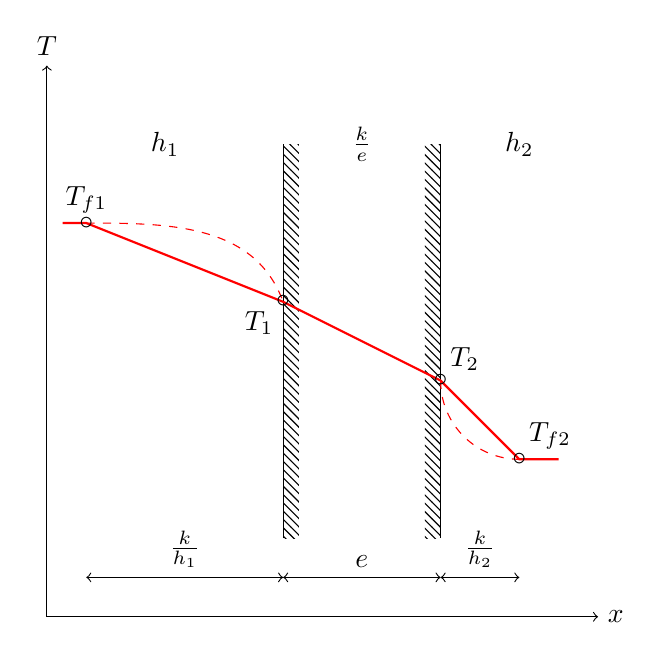
\begin{tikzpicture}
        \draw (0,0) -- (0,5);
    	\fill[pattern=north west lines] (0,0) rectangle ++(0.2,5); 
	    \draw (2,0) -- (2,5);
	    \fill[pattern=north west lines] (2,0) rectangle ++(-0.2,5); 
	    
	    \draw[->] (-3,-1) -- (-3,6) node[above]{$T$};
	    \draw[->] (-3,-1) -- (4,-1) node[right]{$x$};
		\draw[red,thick] (-2.8,4) -- (-2.5,4) -- (0,3) -- (2,2) -- (3,1) -- (3.5,1);
		\draw[red,dashed] (-2.5,4) to[out=0,in=110] (0,3);
		\draw[red,dashed] (2,2) to[out=-90,in=180] (3,1);
		\draw (0,3) node{$\circ$};
		\draw (0,3) node[below left]{$T_1$};
		\draw (2,2) node{$\circ$};
		\draw (2,2) node[above right]{$T_2$};
		\draw (-2.5,4) node{$\circ$};
		\draw (-2.5,4) node[above]{$T_{f1}$};
		\draw (3,1) node{$\circ$};
		\draw (3,1) node[above right]{$T_{f2}$};
		
		\draw[<->] (0,-0.5) -- (2,-0.5) node[midway,above]{$e$};
		\draw[<->] (-2.5,-0.5) -- (0,-0.5) node[midway,above]{$\frac{k}{h_1}$};
		\draw[<->] (2,-0.5) -- (3,-0.5) node[midway,above]{$\frac{k}{h_2}$};
		\draw (-1.5,5) node{$h_1$};
		\draw (1,5) node{$\frac{k}{e}$};
		\draw (3,5) node{$h_2$};
		

    \end{tikzpicture}
    \caption{Distribution de température dans une paroi plane}
    \label{fig:q3_3}
\end{figure}

\subsection{Dérivez l'expression du coefficient de transmission globale $U$ pour une paroi plane composée qui comprend $n$ plaques en contact.}
En pratique on exprime le flux de chaleur $\vec{q}$ en fonction d'un coefficient de transmission $U$ global et des température $T_{f1}$ et $T_{f2}$ :
\begin{equation} \dot{q} = U(T_{f1} - T_{f2}) \end{equation}
Le coefficient $U$ a les mêmes dimensions que $h$. Il s'exprime donc en \si{\watt\per\meter\squared\per\kelvin}. Par la continuité du flux de chaleur on a :
\begin{align} \dot{q} &= h_1(T_{f1}-T_1) = \frac{k_n}{e_n}(T_n-T_{n+1}) = h_2(T_{n+1} - T_{f2}) \\ &= \frac{T_{f1}-T_1}{\frac{1}{h_1}} = \frac{T_1-T_2}{\frac{e_1}{k_1}} = \ldots = \frac{T_n-T_{n+1}}{\frac{e_n}{k_n}} = \frac{T_{n+1}-T_{f2}}{\frac{1}{h_2}} \\ &= \frac{T_{f1}-T_{f2}}{\frac{1}{h_1} + \sum_i^n\frac{e_i}{k_i} + \frac{1}{h_2}} = \frac{T_{f1} - T_{f2}}{\frac{1}{U}}\end{align}
Ceci définit le coefficient de transmission global $U$ :
\begin{equation} \frac{1}{U} = \frac{1}{h_1} + \sum_i^n\frac{e_i}{k_i} + \frac{1}{h_2} \end{equation}

\subsection{Dérivez la distribution de température dans une paroi cylindrique simple. l'étendue de la paroi est infinie, ses surfaces extérieures sont maintenues à des températures constantes et les propriétés de la paroi sont homogènes.}
En régime stationnaire et en l'absence de source volumique de chaleur, l'équation de chaleur \ref{eq:chaleur} se réduit à :
\begin{equation} \grad^2T = 0 \end{equation}
En coordonnées cylindriques cela donne :
\begin{align} \frac{d^2T}{dr^2} + \frac{1}{r}\frac{dT}{dr} = 0 \qquad&\Leftrightarrow\qquad rdT' + T'dr = 0 \\ &\Leftrightarrow\qquad rT' = A \\ &\Leftrightarrow\qquad \frac{dT}{dr} = \frac{A}{r} \end{align}
Par une seconde intégration, on trouve :
\begin{equation} T = A\ln{r} + B \end{equation}
Si nous prenons comme conditions limites
\begin{equation} \begin{cases} T(r=r_i) &= T_i \\ T(r=r_e) &= T_e \end{cases} \qquad \Rightarrow \qquad \begin{cases} T_i &= A\ln{r_i} + B \\ T_e &= A\ln{r_e} + B \end{cases} \end{equation}
on obtient 
\begin{equation} T = \frac{T_i - T_e}{\ln\frac{r_i}{r_e}}\ln{r} + \frac{T_e\ln{r_i} - T_i\ln{r_e}}{\ln\frac{r_i}{r_e}} \label{eq:paroi_cylindrique}\end{equation}
Le profil de température à travers la paroi cylindrique est disponible à la figure \ref{fig:q3_5}
\begin{figure}[p]\centering
	\tikzsetnextfilename{q3_5}
    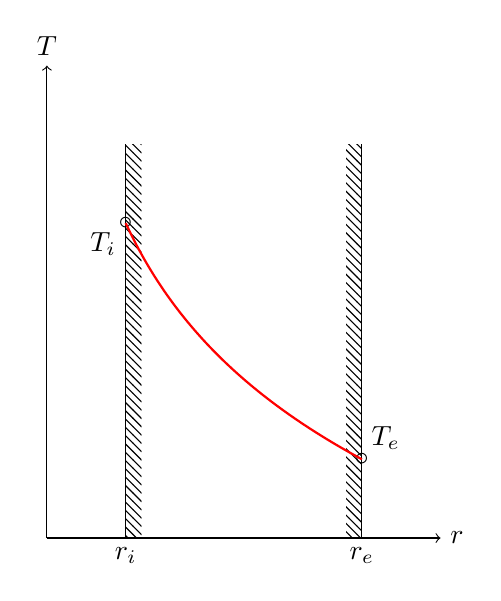
\begin{tikzpicture}
        \draw (1,0) node[below]{$r_i$} -- (1,5);
    	\fill[pattern=north west lines] (1,0) rectangle ++(0.2,5); 
	    \draw (4,0) node[below]{$r_e$} -- (4,5);
	    \fill[pattern=north west lines] (4,0) rectangle ++(-0.2,5); 
	    
	    \draw[->] (0,0) -- (0,6) node[above]{$T$};
	    \draw[->] (0,0) -- (5,0) node[right]{$r$};
		\draw (1,4) node{$\circ$};
		\draw (1,4) node[below left]{$T_i$};
		\draw (4,1) node{$\circ$};
		\draw (4,1) node[above right]{$T_e$};
		
		\draw[domain=1:4,smooth,variable=\x,red,thick] plot ({\x},{-2.164*ln(\x) + 4});
    \end{tikzpicture}
    \caption{Distribution de température dans une paroi cylindrique}
    \label{fig:q3_5}
\end{figure}

\subsection{Dérivez l'expression du rayon critique d'une paroi cylindrique simple}
L'équation explicite du champ thermique à travers une paroi cylindrique \ref{eq:paroi_cylindrique} nous montre que le gradient de température est :
\begin{equation} \grad T = \frac{dT}{dr} = \frac{T_i-T_e}{\ln\frac{r_i}{r_e}}\frac{1}{r} \end{equation}
Le flux, calculé pour une longueur $l$ de la paroi vaut :
\begin{equation} \dot{Q} = S\dot{q} = 2\pi rlk\frac{T_i-T_e}{\ln\frac{r_i}{r_e}}\frac{1}{r} \end{equation}
fa continuité du flux nous indique que celui-ci est indépendant du rayon $r$. En faisant usage des conditions aux frontières :
\begin{equation} \begin{cases} \dot{Q}(r=r_i) &= 2\pi r_ilh_i(T_{fi}-T_i) \\ \dot{Q}(r=r_e) &= 2\pi r_elh_e(T_e-T_{fe}) \end{cases} \end{equation}
où $T_{fi}$ et $T_{fe}$ représente respectivement les températures loin de paroi intérieure et de la paroi extérieure.
On peut exprimer le flux en fonction d'un coefficient de transmission global $U_i$ ou $U_e$ défini par les relations :
\begin{equation} \dot{Q} = U_iS_i(T_{fi}-T_{fe}) = U_eS_e(T_{fi}-T_{fe}) \end{equation}
En effet, on peut écrire :
\begin{equation} \dot{Q} = \frac{T_{fi}-T_i}{\frac{1}{h_iS_i}} = \frac{T_i-T_e}{\frac{1}{2\pi lk}\ln\frac{r_e}{r_i}} = \frac{T_e - T_{fe}}{\frac{1}{h_eS_e}} = \frac{T_{fi}-T_{fe}}{\frac{1}{h_iS_i} + \frac{1}{2\pi lk}\ln\frac{r_e}{r_i} + \frac{1}{h_eS_e}} \end{equation}
Il en résulte donc :
\begin{equation} \frac{1}{U_iS_i} = \frac{1}{U_eS_e} = \frac{1}{h_iS_i} + \frac{1}{2\pi lk}\ln\frac{r_e}{r_i} + \frac{1}{h_eS_e} \end{equation}
On va se concentrer sur $U_i$ mais on peut très bien effectuer un raisonnement similaire sur $U_e$. Si $r_i$, $h_i$ et $h_e$ sont fixés, $1/U_i$ est fonction du rayon extérieur $r_e$ :
\begin{equation} \frac{1}{U_i} = \frac{1}{h_i} + \frac{r_i}{k}\ln\frac{r_e}{r_i} + \frac{1}{h_e}\frac{r_i}{r_e} \end{equation}
Cette fonction se compose de la somme d'un terme constant ($\frac{1}{h_i}$), d'une fonction croissante ($\frac{r_i}{k}\ln\frac{r_e}{r_i}$) et d'une fonction décroissante ($\frac{r_i}{h_er_e}$). Elle présente un minimum pour une valeur de $r_e$ que l'on appelle le rayon critique $r_c$ :
\begin{equation} \frac{d}{dr_e}\left(\frac{1}{U_i}\right) = \frac{r_i}{kr_e} - \frac{r_i}{h_er_e^2} = 0 \qquad \Rightarrow \qquad r_c = \frac{k}{h_e} \end{equation}
Le rayon critique est donc le rayon extérieur pour lequel le flux de chaleur est maximal. 

Envisageons le cas particulier d'un tube isolant placé dans l'air, condition dans laquelle on a normalement $h_e \simeq \SI{10}{\watt\per\meter\squared\per\kelvin}$ et $k \simeq \SI{0.05}{\watt\per\meter\per\kelvin}$. Si on trace la fonction de ($\frac{1}{U_i}$) en fonction de $r_e$ on obtient la figure \ref{fig:q3_6}. Dans le cas d'un tube isolant, on cherche à minimiser la déperdition calorifique. Pour cela on va essayer de rester en deçà du rayon critique en rendant le tube aussi mince que possible. Ce paradoxe provient du fait qu'en diminuant le rayon extérieur, on diminue la résistance liée à la conduction mais on augment aussi celle liée à la convection externe.
\begin{figure}[p]\centering
	\tikzsetnextfilename{rayon_critique_isolant}
    \begin{tikzpicture}
        \begin{axis}[
        	enlargelimits=true,
        	axis lines=left, xtick=\empty, ytick=\empty,
        	grid=major,
        	xmax = 0.025,
        	ymin = -0.02,
        	ylabel=$\frac{1}{U_i}\;(\si{\meter\squared\kelvin\per\watt})$,
        	xlabel=$r_e\;(\si{\meter})$,
        	legend style={font=\footnotesize},
        	xtick={0,0.01,0.015,0.02,0.025},
		    xticklabels={$0$,$1$,$1.5$,$2$,$2.5$},
		    ytick={0,0.05,0.1,0.2},
		    yticklabels={$0$,$0.05$,$0.1$,$0.2$},
    		extra x ticks=0.005,
		    extra x tick style={grid=major, grid style={dashed,black}},
		    extra x tick labels={$r_c$},
    		extra y ticks=0.1522,
		    extra y tick style={grid=major, grid style={dashed,black}},
		    extra y tick labels={$(1/U_1)_\text{min}$}
		]
            \addplot [thick,domain=0.001:0.02,samples=200] {0.1 + 0.02*ln(x/0.001) + 0.0001/x} node[right,pos=1] {$\frac{1}{U_i}$};;
            \addplot [domain=0.001:0.02,samples=200] {0.02*ln(x/0.001)} node[right,pos=1] {$\frac{r_i}{k}\ln\frac{r_e}{r_i}$};
            \addplot [domain=0.001:0.02,samples=200] {0.0001/x} node[right,pos=1] {$\frac{1}{h_e}\frac{r_i}{r_e}$};
        \end{axis}
    \end{tikzpicture}
    \caption{Rayon critique dans le cas d'un tube isolant}
    \label{fig:q3_6}
\end{figure}

\subsection{Dérivez les expressions de deux coefficients de transmission globaux $U_i$ et $U_e$ pour une paroi cylindrique qui se compose de $n$ couches concentriques en contact.}
Si la paroi cylindrique se compose de $n$ couches concentriques en contact, de conductibilités respectives $k_1$, $k_2$, $\ldots$, $k_n$, limitées par les rayons $r_i = r_1$, $r_2$, $\ldots$, $r_n$, $r_{n+1} = r_e$ où $r_i$ désigne le rayon intérieur et $r_e$ le rayon extérieur, on peut écrire pour chaque couche l'expression :
\begin{equation} \dot{Q} = 2\pi lk_j\frac{T_j-T_{j+1}}{\ln\frac{r_{j+1}}{r_j}} \qquad \text{pour } 1\leq j\leq n \end{equation}
De plus, on a :
\begin{equation} \dot{Q} = h_iS_i(T_{fi}-T_1) = h_eS_e(T_{n+1} - T_{fe}) \end{equation}
Dès lors,
\begin{equation} \dot{Q} = \frac{T_{fi}-T_1}{\frac{1}{h_iS_i}} = \ldots = \frac{T_j-T_{j+1}}{\frac{1}{2\pi lk_j}\ln\frac{r_{j+1}}{r_j}} = \ldots = \frac{T_{n+1}-T_{fe}}{\frac{1}{h_eS_e}} = \frac{T_{fi}-T_{fe}}{\frac{1}{U_iS_i}} \end{equation}
On trouve ainsi :
\begin{align} \frac{1}{U_i} &= \frac{1}{h_i} + r_i\sum_j\frac{1}{k_j}\ln\frac{r_{j+1}}{r_j} + \frac{1}{h_e}\frac{r_i}{r_e} \\ \frac{1}{U_e} &= \frac{1}{h_i}\frac{r_e}{r_i} + r_e\sum_j\frac{1}{k_j}\ln\frac{r_{j+1}}{r_j} + \frac{1}{h_e} \end{align}

\subsection{Donnez la définition de débit de capacité calorifique d'un fluide dans un échangeur de chaleur.}
Désignons respectivement par $\dot{M}^x$ et $\dot{M}^0$ les débits massiques des fluides chauffant et chauffé le long de la surface de chauffe, par $T^x$ la température du fluide chauffant et par $T^0$ la température du fluide chauffé. Les indices $1$ et $2$ se rapportent respectivement à l'entrée et à la sortie des fluides dans l'échangeur.

Nous appellerons débit de capacité calorifique d'un fluide le produit $\dot{M}c$ de ce fluide, soit le produit du débit massique et de la capacité calorifique. Les écarts entre $T_1^x$ et $T_2^x$ d'une part, et entre $T_1^0$ et $T_2^0$ d'autre part, sont en pratique suffisamment faibles pour que les chaleurs massiques $c^x$ et $c^0$ puissent être considérées comme constantes.

On considérera également comme constant le coefficient de transmission total à travers la paroi et l'on supposera nulle toute perte calorifique extérieure.

\subsection{Dérivez l'expression pour la distribution de température du fluide chauffant d'un évaporateur co-courant.}
La puissance calorifique $d\dot{Q}$ échangée à travers un élément de surface $dS$ est :
\begin{equation} d\dot{Q} = -\dot{M}^xc^xdT^x = \dot{M}^0c^0dT^0 = U(T^x-T^0)dS \end{equation}
Les signes se justifient par le fait que pour $dS > 0$, on aura $dT^x < 0$ et $dT^0 > 0$. L'évaporateur est un cas particulier d'échangeur de chaleur car la température du fluide chauffé reste constante : $dT^0 = 0$
Dans ce cas, on a :
\begin{equation} \dot{Q} = \dot{M}^xc^x(T_1^x - T_2^x) \end{equation}
et
\begin{equation} \frac{dT^x}{T^x-T^0} = \frac{d(T^x-T^0)}{T^x-T^0} = -\frac{U}{\dot{M}^xc^x}dS \end{equation}
ce qui nous donne :
\begin{align} \ln({T^x-T^0}) &= -\frac{U}{\dot{M}^xc^x}S + C\\
			\Leftrightarrow T^x-T^0 &= C\exp\left(-\frac{U}{\dot{M}^xc^x}S\right) \\
			& \qquad\text{en } S = 0 \text{ on a } T^x-T^0 = T_1^x-T_1^0 \\
			&\Rightarrow C = T_1^x-T^0 \\
			\Leftrightarrow\frac{T^x-T^0}{T_1^x-T^0} &= \exp\left(-\frac{U}{\dot{M}^xc^x}S\right)
\end{align}
Les distributions de température des fluides chauffant $T^x$ et chauffé $T^0$ sont représentées à la figure \ref{fig:q3_9}.
\begin{figure}[p]\centering
	\tikzsetnextfilename{evaporateur_co_courant}
    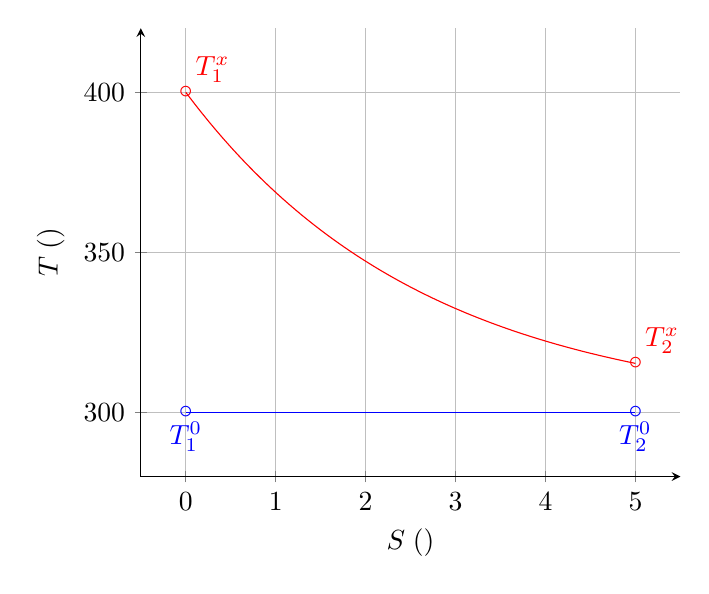
\begin{tikzpicture}
        \begin{axis}[
        	enlargelimits=true,
        	axis lines=left,
        	grid=major,
        	xmin = -0.5, xmax = 5.5,
        	ymin = 280, ymax = 420,
        	ylabel=$T\;(\si{\kelvin})$,
        	xlabel=$S\;(\si{\meter\squared})$,
		]
            \addplot [red,domain=0:5,samples=200] {(100*exp(-0.375*x)) + 300} node[pos=0] {$\circ$} node[above right,pos=0] {$T_1^x$} node[pos=1] {$\circ$} node[above right,pos=1]{$T_2^x$};
            \addplot [blue,domain=0:5,samples=200] {300} node[pos=0] {$\circ$} node[below,pos=0] {$T_1^0$} node[pos=1] {$\circ$} node[below,pos=1]{$T_2^0$};
        \end{axis}
    \end{tikzpicture}
    \caption{Distributions de température dans un évaporateur co-courant}
    \label{fig:q3_9}
\end{figure}

\subsection{Dérivez l'expression pour la distribution de température du fluide chauffé d'un condenseur co-courant.}
La puissance calorifique $d\dot{Q}$ échangée à travers un élément de surface $dS$ est :
\begin{equation} d\dot{Q} = -\dot{M}^xc^xdT^x = \dot{M}^0c^0dT^0 = U(T^x-T^0)dS \end{equation}
Les signes se justifient par le fait que pour $dS > 0$, on aura $dT^x < 0$ et $dT^0 > 0$. Le condenseur est un cas particulier d'échangeur de chaleur car la température du fluide chauffant reste constante : $dT^x = 0$
Dans ce cas, on a :
\begin{equation} \dot{Q} = \dot{M}^0c^0(T_2^0 - T_1^0) \end{equation}
et
\begin{equation} \frac{dT^0}{T^x-T^0} = -\frac{d(T^x-T^0)}{T^x-T^0} = \frac{U}{\dot{M}^0c^0}dS \end{equation}
ce qui nous donne :
\begin{align} \ln({T^x-T^0}) &= -\frac{U}{\dot{M}^0c^0}S + C\\
			\Leftrightarrow T^x-T^0 &= C\exp\left(-\frac{U}{\dot{M}^0c^0}S\right) \\
			& \qquad\text{en } S = 0 \text{ on a } T^x-T^0 = T_1^x-T_1^0 \\
			&\Rightarrow C = T^x-T_1^0 \\
			\Leftrightarrow\frac{T^x-T^0}{T^x-T_1^0} &= \exp\left(-\frac{U}{\dot{M}^0c^0}S\right)
\end{align}
Les distributions de température des fluides chauffant $T^x$ et chauffé $T^0$ sont représentées à la figure \ref{fig:q3_10}.
\begin{figure}[p]\centering
	\tikzsetnextfilename{condenseur_co_courant}
    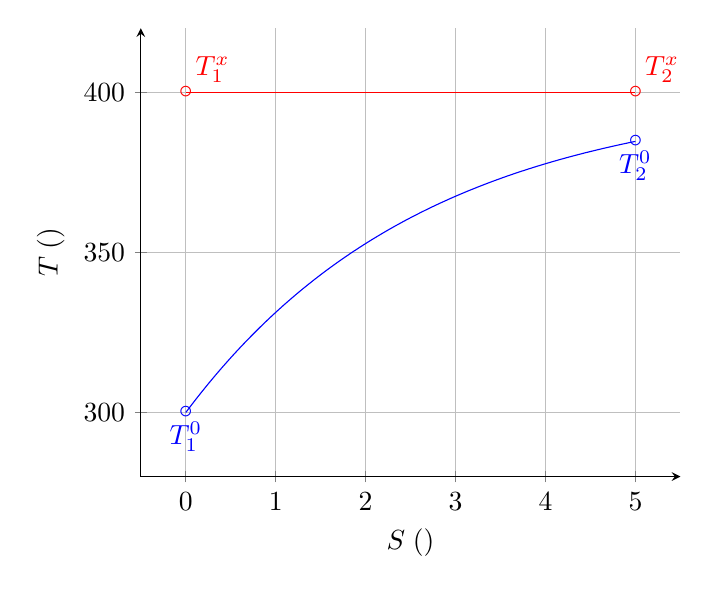
\begin{tikzpicture}
        \begin{axis}[
        	enlargelimits=true,
        	grid=major,
        	axis lines=left,
        	xmin = -0.5, xmax = 5.5,
        	ymin = 280, ymax = 420,
        	ylabel=$T\;(\si{\kelvin})$,
        	xlabel=$S\;(\si{\meter\squared})$,
		]
            \addplot [blue,domain=0:5,samples=200] {-(100*exp(-0.375*x)) + 400} node[pos=0] {$\circ$} node[below,pos=0] {$T_1^0$} node[pos=1] {$\circ$} node[below ,pos=1]{$T_2^0$};
            \addplot [red,domain=0:5,samples=200] {400} node[pos=0] {$\circ$} node[above right,pos=0] {$T_1^x$} node[pos=1] {$\circ$} node[above right,pos=1]{$T_2^x$};
        \end{axis}
    \end{tikzpicture}
    \caption{Distributions de température dans un condenseur co-courant}
    \label{fig:q3_10}
\end{figure}

\subsection{Expliquez le principe de fonctionnement d'un échangeur à fonctionnement non-continu à contact direct.}
\textbf{Un échangeur à fonctionnement non-continu à contact direct} est un échangeur où l'échange calorifique s'obtient par mélange de deux fluides. Le réchauffage d'un liquide peut être réalisé en y injectant de la vapeur, généralement de la vapeur d'eau. Cette méthode n'est applicable que si la condensation de la vapeur n'entraîne pas d'inconvénient pour le liquide. Ce procédé peut être utilisé, par exemple, pour la préparation d'eau chaude, ou pour permettre le déroulement d'une réaction chimique nécessitant une température élevée.

\subsection{Expliquez le principe de fonctionnement d'un échangeur à fonctionnement non-continu et à contact indirect.}
\textbf{Un échangeur à fonctionnement non-continu à contact indirect} est un échangeur dans lequel le liquide est progressivement réchauffé ou refroidi avant d'être évacué. Il existe différents procédés :
\begin{itemize}
\item chauffage électrique (boilers, ceux-ci peuvent aussi fonctionner en régime continu),
\item serpentin immergé dans la cuve dans lequel circule le fluide chauffant ou réfrigérant,
\item cuve à double fond.
\end{itemize}
Dans chacun de ces procédés, il convient d'agiter le fluide afin d'obtenir une répartition uniforme de la température.

\section{Questions sur le chapitre ``Machines thermodynamiques et pertes de charges''}

\section{Questions sur le chapitre ``La thermodynamique des vapeurs''}
\subsection{Donnez les définitions du point critique et du point triple d'une substance. Quel est le nombre de degré de liberté d'une substance au point triple ?}
\begin{description}
\item[Point critique] : le point critique $K$ est le point dans le diagramme ($p$,$v$) d'un fluide vaporisable (Fig. \ref{fig:diag_vdw}) où il n'y a plus de variation de volume lors d'un changement de phase. L'isotherme critique $T_K$ présente un point d'inflexion à tangente horizontale au point $K$. Au-delà de cette température, la seule phase possible est la phase gazeuse.
\item[Point triple] : le point triple $TR$ est le point dans le diagramme ($p$,$T$) d'une substance pure en lequel coexistent les trois phases solide, liquide et gazeuse.
\end{description}
\textbf{La règle des phases de Gibbs} établit une relation entre 
\begin{itemize}
\item $\psi$, le nombre de variables indépendantes intensives déterminant l'état d'un système thermodynamique en équilibre. Ces variables sont aussi appelées degrés de liberté du système;
\item $r$, le nombre de phases;
\item $n$, le nombre de constituants du système.
\end{itemize}
La règle des phases s'exprime par la relation suivante :
\begin{equation} \psi = n - r + 2 \end{equation}
La règle des phases joue un rôle particulièrement important en thermodynamique chimique. Dans le cas d'une substance pure ($n=1$), la règle des phases s'écrit plus simplement :
\begin{equation} \psi = 3 - r \end{equation}
Il en résulte que, pour les substances pures dans un système à une seule phase ($r=1$), le nombre de degrés de liberté est égal à 2. Ces variables indépendantes peuvent être la pression et la température par exemple. 

Au point triple, en $TR$, on a $r=3$, d'où $\psi = 0$. Il n'y a donc aucun degré de liberté lorsque l'on veut atteindre la coexistence des trois phases : un état et un seul est possible en ce point.

\begin{figure}[p]\centering
	\tikzsetnextfilename{diagramme_pv_vdw}
    \begin{tikzpicture}
        \begin{axis}[
        	enlargelimits=true,
        	grid=major,
        	axis lines=left, xtick=\empty, ytick=\empty,
        	xmin = 0.1, xmax = 3.6,
        	ymin = 0.2, ymax = 1.6,
        	ylabel=$p$,
        	xlabel=$v$,
		]
			\addplot [green] table[col sep=comma] {data/vdw1.csv} node[right ,pos=1]{\small$T > T_K$};
			\addplot [green] table[col sep=comma] {data/vdw2.csv};
			\addplot [green] table[col sep=comma] {data/vdw3.csv};
			\addplot [green] table[col sep=comma] {data/vdw4.csv};
			\addplot [red] table[col sep=comma] {data/vdw5.csv} node[right ,pos=1]{\small$T = T_K$};
			\addplot [blue] table[col sep=comma] {data/vdw7.csv};
			\addplot [blue,dashed] table[col sep=comma] {data/vdw8.csv};
			\addplot [blue] table[col sep=comma] {data/vdw9.csv};
			\addplot [blue,dashed] table[col sep=comma] {data/vdw10.csv} node[right ,pos=1]{\small$T < T_K$};
			\addplot [black,thick] table[col sep=comma] {data/vdw6.csv} node[below, pos=0]{\footnotesize Ébullition} node[below,pos=1]{\footnotesize Rosée};
			\draw (1,1) node{$\circ$} node[above]{\small$K$};
			\draw (0.3,0.75) node[fill=white,draw,rectangle]{\small$L$};
			\draw (1.3,0.5) node[fill=white,draw,rectangle]{\small$L+V$};
			\draw (2.7,0.65) node[fill=white,draw,rectangle]{\small$V$};
			\draw (2.5,1.2) node[fill=white,draw,rectangle]{\small$G$};
        \end{axis}
    \end{tikzpicture}
    \caption{Diagramme ($p$,$v$) d'un fluide vaporisable}
    \label{fig:diag_vdw}
\end{figure}
\begin{figure}[p]\centering
	\tikzsetnextfilename{diagramme_phase}
    \begin{tikzpicture}
        \begin{axis}[
        	enlargelimits=true,
        	grid=major,
        	axis lines=left, xtick=\empty, ytick=\empty,
        	xmin = 180, xmax = 310,
        	ymin = -0.2, ymax = 2,
        	ylabel=$p\;(\si{\bar})$,
        	xlabel=$T\;(\si{\kelvin})$,
		]
            \addplot [blue,domain=194.4:216.58,samples=200] {ln(9700000*exp(-26000/(8.314*x)))/ln(10)} node[pos=1]{$\circ$} node[below right, pos=1] {$TR$};
            \addplot [blue,domain=216.6:304.2,samples=200] {ln(0.0000377*x^3 - 0.0217*x^2 + 4.338*x - 299.384)/ln(10)} node[pos=1]{$\circ$} node[right,pos=1]{$K$};
            \addplot [blue,domain=216.1:350,samples=200] {ln(13500*exp(-400/(8.314*(x-210))))/ln(10)};
            \draw (200,1) node[fill=white,draw,rectangle]{\small$S$};
			\draw (260,0.5) node[fill=white,draw,rectangle]{\small$G$};
			\draw (240,1.5) node[fill=white,draw,rectangle]{\small$L$};
        \end{axis}
    \end{tikzpicture}
    \caption{Diagramme ($p$,$T$) d'une substance pure}
    \label{fig:diag_phase}
\end{figure}

\subsection{L'équation d'état de van der Waals est donnée par \ref{eq:vdw}. Expliquez la signification physique des constantes $a$ et $b$ et comment on les obtient à partir des variables d'état au point critique.}
En se basant sur des considérations très simples de théorie cinétique des gaz, van der Waals a proposé l'équation d'état à deux constantes :
\begin{equation} p = \frac{RT}{v-b} - \frac{a}{v^2} \label{eq:vdw} \end{equation}
avec $a$ la force d'attraction intermoléculaire et $b$ le covolume lié au volume propre des molécules, qui n'est négligeable par rapport au volume total que si la pression est faible.  

On calcule ces constantes par l'existence d'un point d'inflexion à tangente horizontale en $K$ pour l'isotherme critique dans un diagramme ($p$,$v$) (Figure \ref{fig:diag_vdw}) : 
\begin{equation} \left.\fpart{p}{v}\right|_{T_K} = 0 \qquad \text{et} \qquad \left.\ffpart{p}{v}\right|_{T_K} = 0 \end{equation}
On réécrit ces conditions sous la forme :
\begin{align} \left.\fpart{p}{v}\right|_{T_K} &= -\frac{RT_K}{(v_K - b)^2} + \frac{2a}{v^3_K} = 0 \\ \left.\ffpart{p}{v}\right|_{T_K} &= \frac{2RT_K}{(v_K - b)^3} - \frac{6a}{v^4_K} = 0 \end{align}
On en déduit :
\begin{equation} v_K = 3b \qquad \text{et} \qquad T_K = \frac{8a}{27Rb} \end{equation}
et l'on trouve par l'équation d'état :
\begin{equation} p_K = \frac{a}{27b^2} \end{equation}

\subsection{Démontrez qu'au point critique la relation \ref{eq:crit} est valable pour un gaz si l'on suit l'équation d'état de van der Waals.}
\begin{equation} \left(\fpart{T}{v}\right)_{p_K} = 0 \label{eq:crit} \end{equation}
Selon l'équation d'état de van der Waals, la température s'exprime de la manière suivante :
\begin{equation} T = \left(p + \frac{a}{v^2}\right)\frac{(v-b)}{R} \end{equation}
On dérive ensuite cette équation :
\begin{equation} \left(\fpart{T}{v}\right)_{p_K} = \left(p_K + \frac{a}{v^2_K}\right)\frac{1}{R} + \left(\frac{v_K-b}{R}\right)\frac{-2a}{v^3_K} \end{equation}
Or au point critique :
\begin{equation} v_K = 3b \qquad \text{et} \qquad p_K = \frac{a}{27b^2} \end{equation}
Et donc :
\begin{align} \left(\fpart{T}{v}\right)_{p_K} &= \left(\frac{a}{27b^2} + \frac{a}{9b^2}\right)\frac{1}{R} + \frac{2b}{R}\left(\frac{-2a}{27b^3}\right) \\ &= \frac{4a}{27b^2R} - \frac{4a}{27b^2R} \\ &= 0 \end{align}

\subsection{Utilisez la relation \ref{eq:crit} ainsi que la propriété générale liant entre elles les chaleurs massiques $c_p$ et $c_v$ pour démontrer qu'au point critique la chaleur massique $c_p$ d'un gaz van der Waals est infinie.}
On sait que (voir question \ref{q:1_7}) :
\begin{align} c_p-c_v &= \alpha\beta pvT \qquad \text{avec} \qquad \alpha = \frac{1}{v}\left(\fpart{v}{T}\right)_p ;\;\beta = \frac{1}{p}\left(\fpart{p}{T}\right)_v \\ &= T\left(\fpart{v}{T}\right)_p\left(\fpart{p}{T}\right)_v \\ &= T\frac{\left(\fpart{p}{T}\right)_v}{\left(\fpart{T}{v}\right)_p} \end{align}
On sait aussi qu'au point critique :
\begin{equation} \left(\fpart{T}{v}\right)_{p_K} = 0 \end{equation}
En admettant que $\left(\fpart{p}{T}\right)_v \neq 0$ (ce qui est vérifiable sur un diagramme ($p$,$T$)) :
\begin{equation} c_p = \infty - c_v = \infty \end{equation}

\subsection{Donnez la définition du ``retard à la vaporisation'' d'un liquide.}
Lorsque l'on décrit une isotherme de température $T<T_K$ en partant soit du liquide, soit de la vapeur, on n'observe pas toujours l'apparition d'une deuxième phase au moment attendu. Il peut y avoir un ``retard à la vaporisation'' : on obtient alors un ``liquide surchauffé'' dont l'isotherme prolonge sans discontinuité celui du liquide. Il peut aussi y avoir un ``retard à la condensation'' : on obtient alors une ``vapeur sursaturée'' dont l'isotherme prolonge sans discontinuité celui de la vapeur sèche. Ces états sont ``métastables''.

\subsection{Dessinez le diagramme ($p$,$v$) d'une isotherme de van der Waals. Quelle est la portion instable dans le tracé. Quelle est la signification d'instabilité ?}
La figure \ref{fig:diag_vdw2} représente le tracé d'une isotherme de van der Waals dans un diagramme ($p$,$v$) : il s'agit d'une cubique qui présente deux extrêmes relatifs en $X$ et en $Y$. Ces états sont instables. En effet, sur cette section, tout accroissement de pression se traduit par une augmentation du volume massique : c'est contraire à l'observation et donc impossible à réaliser.
\begin{figure}[p]\centering
	\tikzsetnextfilename{diagramme_pv_vdw2}
    \begin{tikzpicture}
        \begin{axis}[
        	enlargelimits=true,
        	grid=major,
        	axis lines=left, xtick=\empty, ytick=\empty,
        	xmin = 0.2, xmax = 3.5,
        	ymin = 0.3, ymax = 1.2,
        	ylabel=$p$,
        	xlabel=$v$,
        	xticklabels={,,},yticklabels={,,},
        	extra x ticks={0.6034,2.35},
		    extra x tick style={grid=major, grid style={dashed,black}},
		    extra x tick labels={$v'$,$v''$}
		]
			\addplot [blue] table[col sep=comma] {data/vdw9.csv} node[right ,pos=1]{\small$T = \constant$};
			\addplot [name path=I,restrict expr to domain={x}{0.6034:1.09}, blue,dashed] table[col sep=comma] {data/vdw10.csv};
			\addplot [name path=II,restrict expr to domain={x}{1.09:2.35}, blue,dashed] table[col sep=comma] {data/vdw10.csv};
			\addplot [black,thick] table[col sep=comma] {data/vdw6.csv};
			\path[name path=axis] (0.6034,0.647) -- (2.35,0.647);
			\draw (1,1) node{$\circ$} node[above]{\small$K$};
			\draw (0.6034,0.647) node{$\bullet$} node[left]{$N$};
			\draw (2.35,0.647) node{$\bullet$} node[right]{$M$};
			\draw (1.54,0.724) node{$\bullet$} node[above]{$X$};
			\draw (0.72,0.42) node{$\bullet$} node[below]{$Y$};
			\addplot[blue!30] fill between[of=I and axis];
			\addplot[red!30] fill between[of=II and axis];
			\draw (0.8,0.7) node[fill=blue!30,draw,rectangle]{\small$I$};
			\draw (1.54,0.58) node[fill=red!30,draw,rectangle]{\small$II$};
        \end{axis}
    \end{tikzpicture}
    \caption{Diagramme ($p$,$v$) d'un fluide vaporisable}
    \label{fig:diag_vdw2}
\end{figure}

\subsection{Décrivez et expliquez le processus de réconciliation de la portion instable d'une isotherme produite par l'équation de van der Waals avec les observations expérimentales (reconstruction de Maxwell).}
On remarque que les isothermes obtenues grâce à l'équation d'état de van der Waals ne coïncident pas avec les isothermes représentées sur le diagramme ($p$,$v$) de la figure \ref{fig:diag_vdw2} où l'on remarque que la zone de coexistence entre liquide et vapeur est caractérisée par une isotherme horizontale. En réalité on se situe dans la zone de changement de phase, qu'une équation d'état comme celle de van der Waals ne peut pas décrire correctement. Cependant, le tracé des isothermes de van der Waals peut être réconcilié avec le tracé réel de l'isotherme (la droite horizontale) grâce à la \textbf{construction de Maxwell}.

Les courbes définies par la relation de van der Waals présentent un maximum et minimum local, respectivement en $X$ et $Y$. On remarque que les états représentés sur la courbe allant d'un extremum à l'autre sont instables car un accroissement de pression correspondrait à un accroissement du volume à température constante. Ce qui est impossible à effectuer car
\begin{equation} \left(\fpart{v}{p}\right)_T < 0 \end{equation}
est une des conditions de stabilité thermodynamique.

La construction de Maxwell consiste à remplacer les variations dans la zone de changement de phase par une droite horizontale afin de correspondre aux observations. Cela nécessite d déterminer la pression à laquelle les états liquides et gazeux vont commencer à coexister. C'est-à-dire l'emplacement où l'on va placer l'horizontale. Le long de cette horizontale, liquide et vapeur sont à l'équilibre thermodynamique, ce qui implique que les potentiels chimiques du liquide et de la vapeur sont égaux :
\begin{equation} \mu_A = \mu_B = \constant \qquad \Rightarrow \qquad d\mu = 0 \end{equation}
Ainsi, le changement total du potentiel chimique le long de la courbe $NYXM$ de van de Waals doit aussi être égal à zéro :
\begin{equation} \int_{NYXM}d\mu = 0 \end{equation}
En rappelant que les potentiels chimiques sont fonctions de la température et de la pression, et comme la transformation est une isotherme, la relation de Gibbs-Duhem (\ref{eq:gibbs-duhem}) devient :
\begin{equation} d\mu = vdp - SdT \qquad \Rightarrow \qquad d\mu = vdp \end{equation}
ce qui nous permet de réécrire l'intégrale en séparant par partie le long de la courbe de van der Waals :
\begin{equation} \int_Y^Nvdp + \int_0^Yvdp + \int_X^0vdp + \int_M^Xvdp = 0 \end{equation}
Grâce aux transformations suivantes :
\begin{equation} \int_Y^Nvdp = -\int_N^Yvdp \qquad \text{et} \qquad \int_X^Mvdp = -\int_M^Xvdp \end{equation}
on montre que la droite horizontale représentant l'effet réellement effectué doit se placer de telle sorte que les deux aires soient égales :
\begin{equation} \text{Aire}_{I} - \text{Aire}_{II} = 0 \end{equation}
Comme les deux aires sont égales, on a pour cycle :
\begin{equation} \int_{NYXMN}pdv = 0 \end{equation}
ce qui pemet d'écrire que, en mettant en évidence la pression constance de la ligne horizontale $p_s$ :
\begin{align} p_s(v'-v'') &= \int_{v'}^{v''}pdv \\ \Leftrightarrow p_s &= \frac{1}{(v''-v')}\left(RT\ln\left(\frac{v''-b}{v'-b}\right) + \frac{a}{v''} + \frac{a}{v'}\right) \end{align}
Le calcul des pression de saturation $p_s$ pour des températures différentes permet de tracer les courbes d'ébullition et de rosée. 

\subsection{Donnez la définition du titre d'un mélange liquide/vapeur à l'équilibre.}
Contrairement à l'état gazeux ou liquide, la connaissance d'un couple de valeurs ($p$,$T$) dans le domaine diphasique $L+G$ ne permet pas de connaître complètement l'état thermodynamique. Dans ce cas, il faut introduire une grandeur supplémentaire : le \textbf{titre} $x$, défini comme étant la fraction massique de vapeur dans le mélange liquide/vapeur à l'équilibre. Le titre vaut 0 pour le liquide saturé et vaut 1 pour la vapeur saturée.
\begin{equation} x = \frac{v-v'}{v''-v'} \end{equation}

\subsection{Dérivez la formule de Clapeyron pour la chaleur de vaporisation d'un fluide.\label{q:59}}
Considérons la vaporisation isobare (et donc aussi isotherme) d'un kilo de fluide représentée par les segments $B'B''$ dans les diagrammes ($p$,$v$) et ($T$,$S$) figure \ref{fig:vaporisation}. La chaleur de vaporisation est représentée par la surface $B'B''S''S'$ et peut donc s'exprimer comme suit :
\begin{equation} h_{lv} = \int_{B'}^{B''}TdS = T(S''-S') \end{equation}
Considérons ensuite un cycle $B'C'C''B''$ dont les états $C'$ et $C''$ sont également saturés. Ce cycle correspond à une augmentation $dp$ de la pression et $dT$ de la température. Ce cycle est supposé réversible, les aires dans les 2 diagrammes sont donc égales :
\begin{align} \text{Aire}(p,v) &= (v''-v')dp \\ \text{Aire}(T,S) &= (S''-S')dT = \frac{h_{lv}}{T}dT \end{align}
On en déduit 
\begin{equation} h_{lv} = T(v''-v')\left.\frac{dp}{dT}\right|_\text{sat} \end{equation}
où $\left.\frac{dp}{dT}\right|_\text{sat}$ représente la pente locale de la courbe de pression de vapeur. Cette relation a reçu le nom de \textbf{formule de Clapeyron}.
\begin{figure}[p]\centering
	\tikzsetnextfilename{vaporisation}
    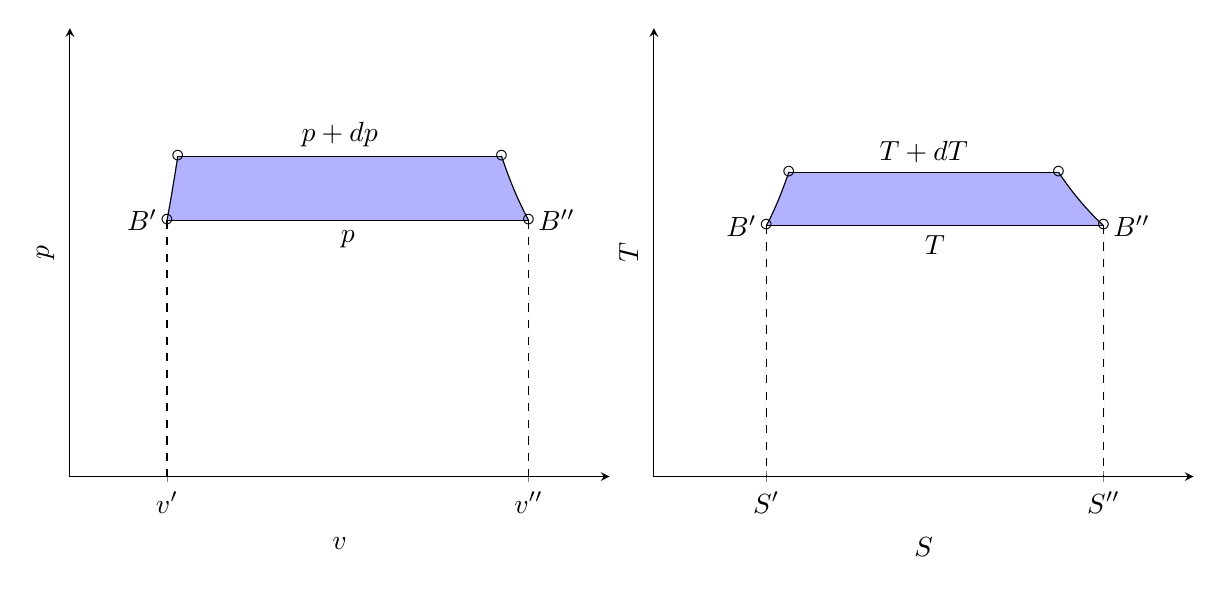
\begin{tikzpicture}
        \begin{axis}[%
    		name=plot1,
    		enlargelimits=true,
        	grid=none,
        	axis lines=left, xtick=\empty, ytick=\empty,
        	xmin = 0, xmax = 10,
        	ymin = -0.5, ymax = 10,
        	ylabel=$p$,
        	xlabel=$v$,
        	no markers,
        	xticklabels={,,},yticklabels={,,},
        	extra x ticks={1.8,8.5},
		    extra x tick labels={$v'$,$v''$}
        ]
        	\addplot+[domain=2:8,fill,blue!30] { 7 } \closedcycle;
        	\addplot+[domain=1.8:2,fill,blue!30] { 3.6111*x*x - 6.2222*x + 5 } \closedcycle;
        	\addplot+[domain=8:8.5,fill,blue!30] { 12.8333/(x-6.16667) } \closedcycle;
        	\addplot+[domain=1.8:8.5,fill,white] { 5.5 } \closedcycle;
        	
        	\addplot[domain=2:8] { 7 };
        	\addplot[domain=1.8:2] { 3.6111*x*x - 6.2222*x + 5 };
        	\addplot[domain=8:8.5] { 12.8333/(x-6.16667) };
        	\addplot[domain=1.8:8.5] { 5.5 };
        	
        	\draw (2,7) node{$\circ$};
        	\draw (8,7) node{$\circ$};
        	\draw[dashed] (1.8,5.5) node{$\circ$} node[left]{$B'$} -- (1.8,-1);
        	\draw[dashed] (8.5,5.5) node{$\circ$} node[right]{$B''$} -- (8.5,-1);
        	\draw (5,7) node[above]{$p+dp$};
        	\draw (5.15,5.5) node[below]{$p$};
    	\end{axis}
        
        \begin{axis}[%
    		name=plot2,
    		at=(plot1.right of south east), anchor=left of south west,
    		axis lines=left, xtick=\empty, ytick=\empty,
    		enlargelimits=true,
        	grid=none,
        	xmin = 0, xmax = 10,
        	ymin = -0.5, ymax = 10,
        	ylabel=$T$,
        	xlabel=$S$,
        	no markers,
        	xticklabels={,,},yticklabels={,,},
        	extra x ticks={1.5,9},
		    extra x tick labels={$S'$,$S''$}
        ]
        	\addplot+[domain=2:8,fill,blue!30] { 7 } \closedcycle;
        	\addplot+[domain=1.5:2,fill,blue!30] { (4/3)*x*x - (5/3)*x + 5 } \closedcycle;
        	\addplot+[domain=8:9,fill,blue!30] { (77/3)/(x-(13/3)) } \closedcycle;
        	\addplot+[domain=1.5:9,fill,white] { 5.5 } \closedcycle;
        	
        	\addplot[domain=2:8] { 7 };
        	\addplot[domain=1.5:2] { (4/3)*x*x - (5/3)*x + 5 };
        	\addplot[domain=8:9] { (77/3)/(x-(13/3)) };
        	\addplot[domain=1.5:9] { 5.5 };
        	
        	\draw (2,7) node{$\circ$};
        	\draw (8,7) node{$\circ$};
        	\draw[dashed] (1.5,5.5) node{$\circ$} node[left]{$B'$} -- (1.5,-2);
        	\draw[dashed] (9,5.5) node{$\circ$} node[right]{$B''$} -- (9,-2);
        	\draw (5,7) node[above]{$T+dT$};
        	\draw (5.25,5.5) node[below]{$T$};
    	\end{axis}
    \end{tikzpicture}
    \caption{Vaporisation isobare (et isotherme) d'un fluide}
    \label{fig:vaporisation}
\end{figure}

\subsection{Calculez la variation d'énergie interne, d'enthalpie et d'entropie le long de l'isotherme liquide $T_0 = \SI{273.15}{\kelvin}$ par rapport à l'état du liquide saturé à $T_0$.}
L'état de référence choisi est celui du liquide saturé à $T_0$, représenté par le point $A_0$ de la figure \ref{fig:T0ref}. Désignons par $p_0$ la pression et $v_0$ le volume massique à l'état de référence. Les symboles $U_0$, $H_0$ et $S_0$ désignent les fonctions d'état à l'état de référence choisi. Nous pouvons dès lors définir les variations par rapport au point $A$ de l'énergie interne $u_A$, de l'enthalpie $h_A$ et de l'entropie $s_A$ que nous allons calculer par les relations respectives suivantes:
\begin{equation} u_A = U_A-U_{0} \qquad h_A = H_A-H_{0} \qquad s_A = S_A-S_{0} \end{equation}
l'état $A$ étant défini par la pression $p$ et la température $T_0$ (sur la même isotherme que $A_0$). L'étude du comportement de la substance à l'état liquide autour de $T_0=\SI{273.15}{\kelvin}$, plus particulièrement en ce qui concerne les coefficients de dilatation et de compressibilité, permet d'établir une équation d'état du liquide :
\begin{equation} v = v(T,p) \end{equation}
\paragraph{Entropie} En se rappelant que l'enthalpie libre de Gibbs $G$ est une fonction d'état, telle que :
\begin{equation} dG = -SdT + vdp \end{equation}
on déduit, par le théorème de Schwarz :
\begin{equation} -\left.\fpart{S}{p}\right|_T = \left.\fpart{v}{T}\right|_p = \alpha v \qquad \text{avec} \qquad \alpha = \frac{1}{v}\left(\fpart{v}{T}\right)_p \end{equation}
ce qui permet de calculer la varation d'entropie le long de l'isotherme $T_0$. En intégrant, on trouve :
\begin{equation} s_A = S_A-S_0 = -\int_{p_0}^{p_A}\alpha vdp = -\overline{\alpha v}(p_A-p_0) \end{equation}
où $\overline{\alpha v}$ représente la valeur moyenne de $\alpha v$ sur l'intervalle $\left[p_0,p_A\right]$. Les facteurs $\alpha$ et $v$ sont très petits, de l'ordre de $10^{-3}$ chacun pour l'eau. Il est dès lors raisonnable de négliger la valeur de leur produit et de retenir :
\begin{equation} s_A \simeq 0 \end{equation}
\paragraph{Énergie interne} La variation de $U$ est donnée par :
\begin{equation} dU = TdS - pdv \simeq -pdv \end{equation}
et donc :
\begin{equation} u_A = U_A - U_0 \simeq -\overline{p}(v_0-v_A) \end{equation}
Le volume massique n'évoluant que très peu avec la pression (le coefficient de compressibilité est de l'ordre de $10^{-4}$ pour l'eau). Il est, ici aussi, raisonnable de retenir :
\begin{equation} u_A \simeq 0 \end{equation}
\paragraph{Enthalpie} Le calcul de l'enthalpie est aisé. Par $H = U + pv$, on trouve immédiatement :
\begin{equation} h_A = H_A-H_0 = v_0(p_A-p_0) \end{equation}
Il s'agit d'une petite quantité, mais pas négligeable pour autant.
\begin{figure}[p]\centering
	\tikzsetnextfilename{T0ref}
    \begin{tikzpicture}
        \begin{axis}[
        	enlargelimits=true,
        	%grid=major,
        	axis lines=left, xtick=\empty, ytick=\empty,
        	xmin = 0.3, xmax = 3.4,
        	ymin = 0.3, ymax = 1.2,
        	ylabel=$p$,
        	xlabel=$v$,
        	xticklabels={,,},yticklabels={,,},
        	extra x ticks={0.6841,1.727},
		    extra x tick style={grid=major, grid style={dashed,black}},
		    extra x tick labels={$v'$,$v''$},
		    extra y ticks={0.8119},
		    extra y tick style={grid=major, grid style={dashed,black}},
		]
			\addplot [blue] table[col sep=comma] {data/vdw9.csv};
			\addplot [blue] table[col sep=comma] {data/vdw7.csv};
			\addplot [black,thick] table[col sep=comma] {data/vdw6.csv};
			\path[name path=axis] (0.6034,0.647) -- (2.35,0.647);
			\draw (1,1) node{$\circ$} node[above]{\small$K$};
			\draw[blue] (1.3,0.647) node[above]{$T_0$};
			\draw (0.6034,0.647) node{$\bullet$} node[left]{$A_0$};
			\draw (0.58,0.8119) node{$\bullet$} node[above left]{$A$};
			\draw (0.6841,0.8119) node{$\bullet$} node[above right]{$B'$};
			\draw (1.727,0.8119) node{$\bullet$} node[above right]{$B''$};
        \end{axis}
    \end{tikzpicture}
    \caption{Diagramme ($p$,$v$) d'un fluide vaporisable}
    \label{fig:T0ref}
\end{figure}

\subsection{Calculez les valeurs d'énergie interne $u'$, d'enthalpie $h'$ et d'entropie $s'$ pour les états de liquide saturé, ainsi que les valeurs d'énergie interne $u''$, d'enthalpie $h''$ et d'entropie $s''$ pour les états de vapeur saturé.}
Nous considérons ici la transformation isobare $AB'$ de la figure \ref{fig:T0ref}. On a :
\begin{equation} h' - h_A = q_\text{éch} = \int_{273.15}^Tc_{pl}dT \end{equation}
où $q_\text{éch}$ est la chaleur d'échauffement du liquide, l'action calorifique requise pour augmenter, sous pression constante, la température du liquide de $\SI{0}{\celsius}$ jusqu'à la température de saturation $t_\text{sat}$. Le calcul de sa valeur nécessite la détermination de celle de la chaleur massique $c_{pl}$ du liquide qui varie avec la pression et la température.
On a ensuite :
\begin{equation} u' - u_A = h' - h_A - p_A(v'-v_A) \end{equation}
d'où :
\begin{align} u' &= h' - (p_Av' - p_0v_0) \\ s'-s_A = s' &= \int_{273.15}^T\frac{c_{pl}}{T}dT \end{align}
Le calcul des valeurs $u''$, $h''$ et $s''$ pour les états de vapeur saturée est immédiat :
\begin{align} h''-h' &= h_{lv} \\ s''-s' &= \frac{h''-h'}{T_\text{sat}} = \frac{h_{lv}}{T_\text{sat}} \\ u''-u' &= h_{lv} - p(v''-v') \end{align}
où $h_{lv}$ est la chaleur de vaporisation, définie à la question \ref{q:59}.

\section{Questions sur le chapitre ``Machine de compression''}

\section{Questions sur le chapitre ``Machine de détente''}

\section{Questions sur le chapitre ``L'air humide''}

\section{Questions sur le chapitre ``Turbines à gaz et cycles à vapeurs''}
\subsection{Dessinez un cycle thermodynamique idéal d'une turbine à gaz sur les plans $(p,v)$ et $(T,s)$. Décrivez les 4 étapes du cycle.}
Le cycle de Brayton, aussi connu sous le nom de cycle de Joule, est le cycle idéal correspondant à la turbine à gaz élémentaire. Il existe deux types de cycles de Brayton selon qu'il soit ouvert, ou refermé sur l'atmosphère en utilisant un échangeur de chaleur. C'est la première variante qui retiendra notre attention puisque c'est celle qui est utilisée dans les centrales électriques Turbines Gaz Vapeurs (TGV). Le cycle est constitué de quatre étapes (voir Figure \ref{fig:cycleTG}):
\begin{description}
	\item[1 $\rightarrow$ $\mathbf{2_S}$] Compression de l'air au moyen d'un compresseur.
	\item[$\mathbf{2_S}$ $\rightarrow$ 3] L'air comprimé est chauffé dans la chambre de combustion lors d'un processus isobare.
	\item[3 $\rightarrow$ $\mathbf{4_S}$] Détente des fumées au moyen d'une turbine.
	\item[$\mathbf{4_S}$ $\rightarrow$ 1] Rejet des fumées dans l'atmosphère.
\end{description} 
Compresseur, turbine et alternateur sont sur le même arbre. C'est donc la turbine qui entraîne le compresseur at l'alternateur. Dans un cycle idéal, la compression et la détente sont supposées isentropiques tandis que la combustion est supposée isobare.
\begin{figure}[p]\centering 
	\tikzsetnextfilename{cycleTG}
	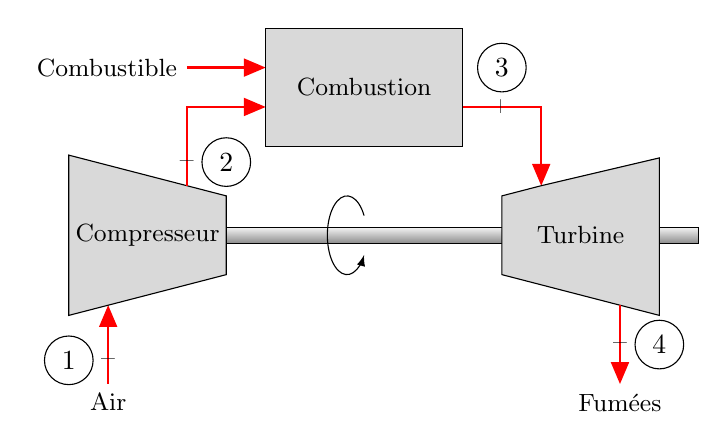
\begin{tikzpicture}
		\draw[top color=gray!10, bottom color=gray!90] (1.5,{1.4+1.5*sin(15)}) rectangle (7.5,{1.6+1.5*sin(15)});
		\draw[-triangle 45,red,thick] (0,0) -- (0,1);
		\draw[fill=gray!30] (-0.5,{1-0.5*sin(15)}) -- ++(2,{2*sin(15)}) -- ++(0,1) -- ++(-2,{2*sin(15)}) --cycle;
		\draw[-triangle 45,red,thick] (1,{2+2*sin(15)}) |- ++(1,1) coordinate (A);
		\draw[-triangle 45,red,thick] (1,{3.5+2*sin(15)}) -- (2,{3.5+2*sin(15)}); 
		\draw[fill=gray!30] (A) -- ++(0,1) -- ++(2.5,0) -- ++(0,-1) coordinate (B) -- ++(0,-0.5) -- ++(-2.5,0) --cycle;
		\draw[-triangle 45,red,thick] (B) -| ++(1,-1) coordinate (C);
		\draw[fill=gray!30] (C) -- ++(-0.5,-{0.5*sin(15)}) -- ++(0,-1) -- ++(1.5,{-1.5*sin(15)}) coordinate (D) -- ++(0.5,{-0.5*sin(15)}) -- ++(0,2) --cycle;
		\draw[-triangle 45,red,thick] (D) -- ++(0,-1);
		\draw (-0.5,0.3) node[draw,circle]{1};
		\draw (0,0.3) node{--};
		\draw (0,0) node[below]{\small Air};
		\draw (0.5,{1.5+1.5*sin(15)}) node{\small Compresseur};
		\draw (1.5,{2+2*sin(15)+0.3}) node[draw,circle]{2};
		\draw (1,{2+2*sin(15)+0.3}) node{--};
		\draw (1,{3.5+2*sin(15)}) node[left]{\small Combustible};
		\draw (3.25,{3.25+2*sin(15)}) node{\small Combustion};
		\draw (5,{3+2*sin(15)+0.5}) node[draw,circle]{3};
		\draw (5,{3+2*sin(15)}) node[rotate=90]{--};
		\draw (6,{1.5+1.5*sin(15)}) node{\small Turbine};
		\draw (6.5,0.5) node{--};
		\draw (7,0.5) node[draw,circle]{4};
		\draw (6.5,0) node[below]{\small Fumées};
		\draw[-latex] (3.25,{1.75+1.5*sin(15)}) arc (30:330:0.25 and 0.5);
	\end{tikzpicture}
	\tikzsetnextfilename{pvcycleTG}
    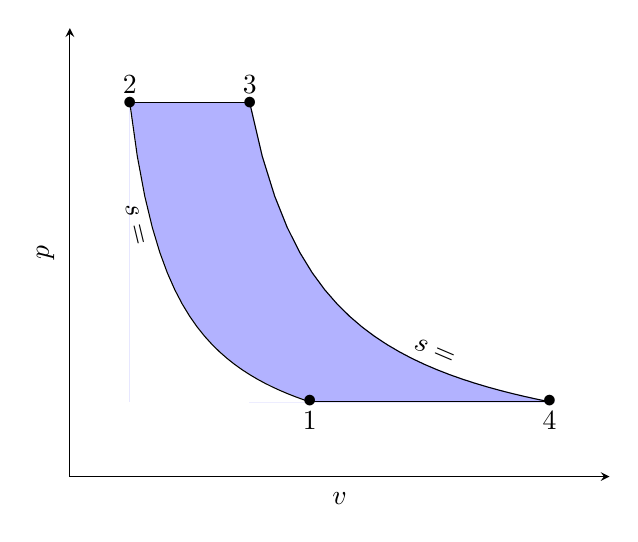
\begin{tikzpicture}
        \begin{axis}[%
    		enlargelimits=true,
        	grid=none,
        	axis lines=left, xtick=\empty, ytick=\empty,
        	xmin = 0, xmax = 9,
        	ymin = -1, ymax = 5,
        	ylabel=$p$,
        	xlabel=$v$,
        	no markers,
        ]        	
        	\addplot+[domain=1:3,fill,blue!30] { 4 } \closedcycle;
        	\addplot+[domain=3:8,fill,blue!30] { 6.25/(x-1.75) - 1} \closedcycle;
        	\addplot+[domain=1:4,fill,white] { 3.75/(x-0.25) - 1 } \closedcycle;
        	\addplot+[domain=4:8,fill,white] { 0 } \closedcycle;
        	\addplot[domain=1:3] { 4 };
        	\addplot[domain=3:8] { 6.25/(x-1.75) - 1 } node[pos=0.7,sloped,above]{$s=\constant$};
        	\addplot[domain=1:4] { 3.75/(x-0.25) - 1 } node[pos=0.3,sloped,below]{$s=\constant$};;
        	\addplot[domain=4:8] { 0 };
        	
        	\draw (4,0) node{$\bullet$} node[below]{1};
        	\draw (1,4) node{$\bullet$} node[above]{2};
        	\draw (3,4) node{$\bullet$} node[above]{3};
        	\draw (8,0) node{$\bullet$} node[below]{4};
    	\end{axis}
    \end{tikzpicture}
    \tikzsetnextfilename{TScycleTG}
    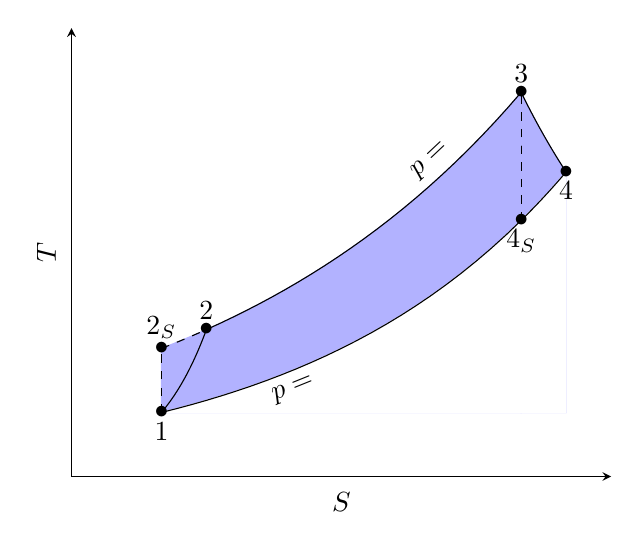
\begin{tikzpicture}
        \begin{axis}[%
    		enlargelimits=true,
        	grid=none,
        	axis lines=left, xtick=\empty, ytick=\empty,
        	xmin = 0, xmax = 6,
        	ymin = -1, ymax = 6,
        	ylabel=$T$,
        	xlabel=$S$,
        	no markers,
        ]        	
        	\addplot+[domain=1:5,fill,blue!30] { 1.5197*1.3161^x - 1 } \closedcycle;
        	\addplot+[domain=5:5.5,fill,blue!30] { 87.1945*0.5645^x } \closedcycle;
        	\addplot+[domain=1:5.5,fill,white] { 0.7071*1.4142^x - 1 } \closedcycle;
        	\addplot[dashed,domain=0:1] (1,x);
        	\addplot[dashed,domain=1:1.5] { 1.5197*1.3161^x - 1 };
        	\addplot[domain=1.5:5] { 1.5197*1.3161^x - 1 } node[pos=0.7,sloped,above]{$p=\constant$};
        	\addplot[domain=5:5.5] { 87.1945*0.5645^x };
        	\addplot[domain=1:5] { 0.7071*1.4142^x - 1 } node[pos=0.3,sloped,below]{$p=\constant$};
        	\addplot[domain=5:5.5] { 0.7071*1.4142^x - 1 };
        	\addplot[domain=1:1.5] { 0.1899*5.2647^x - 1 };
        	\addplot[dashed,domain=3:5] (5,x);
        	
        	\draw (1,0) node{$\bullet$} node[below]{1};
        	\draw (1,1) node{$\bullet$} node[above]{$2_S$};
        	\draw (1.5,1.2945) node{$\bullet$} node[above]{2};
        	\draw (5,3) node{$\bullet$} node[below]{$4_S$};
        	\draw (5.5,3.7568) node{$\bullet$} node[below]{$4$};
        	\draw (5,5) node{$\bullet$} node[above]{3};
    	\end{axis}
    \end{tikzpicture}
	\caption{Schéma de principe et diagrammes ($p$,$v$) et ($T$,$S$) d'une turbine à gaz}
	\label{fig:cycleTG}
\end{figure}

\subsection{On considère le cycle d'une turbine à gaz. On suppose que $p_2 = p_3$, que $c_p = C^\text{te}$ et que les flux de masse à la turbine et au compresseur sont égaux. Dérivez l'expression du rendement thermique du cycle.}
L'expansion thermique des gaz due à l'effet de la source chaude donne lieu à la production d'une puissance motrice de détente supérieure à celle nécessaire à la compression du gaz frais. La puissance effective $P_e$ de cette installation peut s'écrire :
\begin{equation} P_e = \underbrace{P_{mT}}_{\text{turbine}} - \underbrace{P_{mC}}_{\text{compresseur}} - \underbrace{P_{fm+aux}}_{\text{frottements mécaniques et auxilliaires}} \end{equation} 
En désignant $\dot{m}_T$ et $\dot{m}_C$ les flux de masse à la turbine et au compresseur, il vient encore :
\begin{equation} P_e = \dot{m}_TW_{mT} - \dot{m}_CW_{mC} - P_{fm+aux} \end{equation}
On peut donc définir la puissance motrice 
\begin{equation} P_m = P_e + P_{fm+aux} = \dot{m}_TW_{mT} - \dot{m}_CW_{mC} \end{equation}
Le travail moteur de l'installation s'exprime donc :
\begin{equation} W_m = \frac{P_m}{\dot{m}_C} = \frac{\dot{m}_T}{\dot{m}_C}W_{mT}-W_{mC} \end{equation}
En prenant en compte les hypothèses simplificatrices habituelles d'identité des états d'énergie cinétique et d'énergie potentielle en chacun des point remarquables du cycle ($\Delta k = \Delta z = 0$) ainsi que le caractère adiabatique des transformations de compression et de détente, nous obtenons :
\begin{align} W_{mT} &= -\int^4_3vdp - W_{fT} = h_3-h_4 \\ W_{mC} &= \int^2_1vdp + W_{fC} = h_2-h_1 \end{align}
Étant donné que les flux de masse à la turbine et au compresseur sont égaux ($\dot{m}_T = \dot{m}_C$), que $c_p$ est constant et que $p_2 = p_3$, le travail moteur s'écrit  
\begin{equation} W_m = (h_3-h_4) - (h_2-h_1) = c_p\left((T_3-T_4) - (T_2-T_1)\right)\end{equation}
Avec toutes les hypothèses, la chaleur fournie lors de la combustion $Q$ correspond à 
\begin{equation} Q = \Delta^3_2h \end{equation}
On trouve donc l'expression du rendement thermique du cycle :
\begin{equation} \eta_{th} = \frac{W_m}{Q} = \frac{c_p((T_3-T_4)-(T_2-T_1))}{c_p(T_3-T_2)} = \frac{T_3-T_2-T_4+T_1}{T_3-T_2} = 1 - \frac{T_4-T_1}{T_3-T_2} \label{eq:q4_3}\end{equation}

\newcommand{\sit}{\eta_\text{SiT}}
\newcommand{\sic}{\eta_\text{SiC}}
\subsection{À partir de l'expression \ref{eq:q4_3}, dérivez l'expression du rendement thermique $\eta_\text{th}$ d'une turbine à gaz en fonction du rendement isentropique interne $\sic$ du compresseur et $\sit$ de la turbine.} 
L'introduction des notions de rendement isentropique interne $\sic$ de la compression et $\sit$ de la turbine nous permet de réécrire l'équation du travail moteur :
\begin{align} W_m &= \sit c_p(T_3-T_{4S})-\frac{1}{\sic}c_p(T_{2S}-T_1) \\ &= \sit c_pT_3\left(1-\frac{T_{4S}}{T_3}\right)-\frac{1}{\sic}c_pT_1\left(\frac{T_{2S}}{T_1}-1\right)\end{align}
et celle de l'effet calorifique fourni par la combustion :
\begin{align} Q_I &= c_p(T_3-T_2) \\ &= c_p(T_3-(T_2-T_1)-T_1) \\ &= c_p\left(T_3-T_1-\frac{1}{\sic}(T_{2S}-T_1)\right) \end{align}
Les états $2S$ et $4S$ sont ceux qui seraient atteint respectivement en fin de compression et de détente adiabatiques sans travaux dissipatifs (voir figure \ref{fig:cycleTG}). Pour simplifier l'écriture, on pose :
\begin{equation} X \triangleq \left(\frac{p_2}{p_1}\right)^{\frac{\gamma-1}{\gamma}} = \left(\frac{p_3}{p_4}\right)^{\frac{\gamma-1}{\gamma}} = \frac{T_{2S}}{T_1} = \frac{T_3}{T_{4S}} \label{eq:Xcomp}\end{equation}
qui est une image non linéaire du rapport de pression réalisé dans la machine. On introduit aussi le rapport entre la température maximale du fluide moteur et la température de base du cycle\footnote{On exprime par ce paramètre $Y$ la contrainte thermique à laquelle sera astreinte la turbine. Il est impératif de conserver à chaud la tenue mécanique et les qualités aérodynamiques des ailettes, ce qui conduit à limiter $T_3$ en pratiquant pour la combustion un coefficient d'excès d'air adéquat.} , à savoir :
\begin{equation} Y \triangleq \frac{T_3}{T_1} \label{eq:Ytemp}\end{equation} 
L'utilisation des paramètres $X$ et $Y$ conduit aux relations adimensionnelles :
\begin{align} \frac{W_m}{c_pT_1} &= \sit Y\left(1-\frac{1}{X}\right) - \frac{1}{\sic}\left(X-1\right) \\ &= \left(\sit\frac{Y}{X}-\frac{1}{\sic}\right)(X-1) \end{align}
et 
\begin{align} \frac{Q_I}{c_pT_1} &= Y - 1 - \frac{1}{\sic}(X-1) \end{align} 
On tire de ces expressions celle du rendement thermique $\eta_{th}$ en fonction de $\sic$ et $\sit$:
\begin{equation} \eta_{th} = \frac{W_m}{Q_I} = \frac{\left(\sit\frac{Y}{X}-\frac{1}{\sic}\right)(X-1)}{Y - 1 - \frac{1}{\sic}(X-1)} \end{equation}

\newcommand{\pit}{\eta_\text{piT}}
\newcommand{\pic}{\eta_\text{piC}}
\subsection{À partir de l'expression \ref{eq:q4_3}, dérivez l'expression du rendement thermique $\eta_\text{th}$ d'une turbine à gaz en fonction du rendement polytropique $\pic$ du compresseur et $\pit$ de la turbine.\label{q:9.4}}
On réécrit l'équation du travail moteur :
\begin{equation} W_m = c_pT_3\left(1-\frac{T_4}{T_3}\right) - c_pT_1\left(\frac{T_2}{T_1}-1\right) \end{equation}
et celle de l'effet calorifique fourni par la combustion :
\begin{equation} Q_I = c_pT_1\left(\frac{T_3}{T_1}-\frac{T_2}{T_1}\right)\end{equation}
Le recours au modéle polytropique du fonctionnement des turbomachines pour décrire les transformation qui s'y produisent avec travaux dissipatifs $W_f$ conduit à utiliser les rendements polytropiques $\pic$ du compresseur et $\pit$ de la turbine tels que l'on ait :
\begin{align} \frac{T_2}{T_1} &= \left(\frac{p_2}{p_1}\right)^{\frac{m-1}{m}} = \left(\frac{p_2}{p_1}\right)^{\frac{\gamma-1}{\gamma}\frac{1}{\pic}} = \left(\frac{T_{2S}}{T_1}\right)^{\frac{1}{\pic}} = X^{\frac{1}{\pic}} \\ \frac{T_4}{T_3} &= \left(\frac{p_4}{p_3}\right)^{\frac{m-1}{m}} = \left(\frac{p_4}{p_3}\right)^{\frac{\gamma-1}{\gamma}\pit} = \left(\frac{T_{4S}}{T_3}\right)^{\pit} = \left(\frac{1}{X}\right)^{\pit} \end{align}
avec $m$ l'indice polytropique, $\gamma$ l'indice adiabatique, $T_{2S}$ et $T_{4S}$ les températures aux états $2S$ et $4S$ qui seraient atteint respectivement en fin de compression et de détente adiabatiques sans travaux dissipatifs $W_f$ et $X$ l'image non linéaire du rapport de pression réalisé dans la machine défini par l'équation \ref{eq:Xcomp}. On conserve le paramètre $Y$ défini par l'équation \ref{eq:Ytemp}. L'utilisation des paramètres $X$ et $Y$ conduit aux relations adimensionnelles :
\begin{align} \frac{W_m}{c_pT_1} &= Y\left(1-\frac{1}{X^{\pit}}\right) - X^{\frac{1}{\pic}} + 1 \\ \frac{Q_I}{c_pT_1} &= Y - X^{\frac{1}{\pic}} \end{align}
On tire de ces expression celle du rendement thermique $\eta_{th}$ en fonction de $\pic$ et $\pit$ :
\begin{equation} \eta_{th} = \frac{W_m}{Q_I} = \frac{Y\left(1-\frac{1}{X^{\pit}}\right) - X^{\frac{1}{\pic}} + 1}{Y - X^{\frac{1}{\pic}}} \end{equation}


\subsection{À partir de l'expression \ref{eq:q4_5}, dérivez l'expression du travail moteur $W_m$ d'une turbine à gaz en fonction du rendement isentropique interne $\eta_\text{SiC}$ du compresseur et $\eta_\text{SiT}$ de la turbine. Pour un rapport de température \ref{eq:q4_52} fixé, calculer les valeurs du rapport de compression \ref{eq:q4_53} qui annulent $W_m$.}
\begin{equation} \label{eq:q4_5} W_m = c_p\left(\left(T_3-T_4\right) - \left(T_2-T_1\right)\right) \end{equation}
\begin{equation} \label{eq:q4_52} Y = \frac{T_3}{T_1} \end{equation}
\begin{equation} \label{eq:q4_53} X = \left(\frac{p_2}{p_1}\right)^\frac{(\gamma-1)}{\gamma} \end{equation}

On peut réécrire l'équation \ref{eq:q4_5} en y introduisant les rendements isentropiques internes des turbomachines :
\begin{equation} W_m = c_pT_3\left(1-\frac{T_4}{T_3}\right) - c_pT_1\left(\frac{T_2}{T_1} - 1\right) = \sit c_pT_3\left(1-\frac{T_{4S}}{T_3}\right) - \frac{1}{\sic}c_pT_1\left(\frac{T_{2S}}{T_1} - 1\right) \end{equation}
Le paramètre $X$ peut aussi s'écrire :
\begin{equation} X \triangleq \left(\frac{p_2}{p_1}\right)^\frac{(\gamma-1)}{\gamma} = \frac{T_3}{T_{4S}} = \frac{T_{2S}}{T_{1}} \end{equation}
On a donc :
\begin{equation} \frac{W_m}{c_pT_1} = \left(\sit\frac{Y}{X}-\frac{1}{\sic}\right)(X-1) \end{equation}
On observe que le travail moteur s'annulent en $X=1$ et en $X = X_0$ de valeur :
\begin{equation} X_0 = \sic\sit Y \end{equation}

\subsection{À partir de l'expression \ref{eq:q4_5}, dérivez l'expression du travail moteur $W_m$ d'une turbine à gaz en fonction du rendement polytropique $\eta_\text{piC}$ du compresseur et $\eta_\text{piT}$ de la turbine. Dérivez également le maximum de $W_m$ en fonction du rapport de compression \ref{eq:q4_53}.}
L'étape de dérivation de l'expression du travail moteur $W_m$ en fonction des rendements polytropiques $\pic$ et $\pit$ a déjà été développée à la section \ref{q:9.4} :
\begin{equation} \frac{W_m}{c_pT_1} = Y\left(1-\frac{1}{X^{\pit}}\right) - X^{\frac{1}{\pic}} + 1 \end{equation}
On trouve la valeur maximale de $W_m$ selon $X$ en annulant sa dérivée selon $X$ :
\begin{align} \fpart{}{X}\left(Y\left(1-\frac{1}{X^{\pit}}\right) - X^{\frac{1}{\pic}} + 1\right) &= 0 \\ \pit YX^{-\pit-1} - \frac{X^{\frac{1}{\pic}-1}}{\pic} &= 0 \\ X^{\pit+\frac{1}{\pic}} &= \pit\pic Y \\ X_A &= \left(\pit\pic Y\right)^{\frac{1}{\frac{1}{\pic}+\pit}} \simeq \sqrt{\pit\pic Y} \end{align}
où $X_A$ correspond à la valeur pour laquelle $W_m$ passe par un maximum. On remarque que $X_A$ est une fonction croissante de $Y$.


\subsection{Dans l'utilisation des turbines à gaz essaye-t-on de maximiser le travail effectif, $W_e$, ou le rendement effectif, $\eta_e$. Justifiez votre réponse.}
On rappelle que le rendement effectif est défini par $\eta_e \triangleq \eta_{th}\eta_{mec}$ et le travail effectif par $W_e \triangleq \eta_{mec}W_m$.
Soit $X_A$ le rapport de compression qui maximise le travail moteur et $X_B$ celui qui maximise le rendement thermique. Le maximum du rendement effectif correspond à une valeur $X_M$ telle que l'on ait toujours :
\begin{equation} X_A \leq X_M \leq X_B \end{equation} 
On observe en pratique que :
\begin{itemize}
\item la variation relative du rendement effectif est moindre que celle du travail effectif dans l'intervalle $X_A \leq X_M \leq X_B$. Il est donc plus pénalisant pour le travail effectif de choisir le point $X_B$ qu'il n'est pénalisant pour le rendement de choisir le point $X_A$;
\item en termes de rapport de pression, le fonctionnement à rendement maximum est de loin plus exigeant que le fonctionnement à travail moteur maximum et implique le recours à une technologie plus coûteuse tant pour le compresseur (nombre élevé d'étages) que pour la chambre de combustion (haute densité de puissance thermique).
\end{itemize}
On utilisera donc en pratique un rapport de compression plus proche de celui donnant lieu au maximum de travail que celui conduisant au maximum du rendement.

\subsection{Donnez la définition d'exergie dans une installation à cycle combiné et expliquez sa signification physique.}
Une installation à cycle combiné profite de la température encore élevée des gaz d'échappement pour produire du travail moteur par un cycle thermique en aval de la turbine à gaz. En pratique il s'agit d'un cycle utilisant la détente dans une turbine de la vapeur sous pression produite par une chaudière grâce à la récupération d'une fraction de l'enthalpie sensible des gaz d'échappement (voir exemple figure \ref{fig:cycleTGCAV}). Si l'on désigne par $\eta_R$ le taux de récupération de cette enthalpie sensible, qui représente pour la turbine à gaz la perte à la source froid $1-\eta_{TG}$, tandis que $\eta_{CAV}$ désigne le rendement de conversion en travail de la chaleur ainsi récupérée, le rendement global de conversion de la chaleur en travail moteur a pour valeur dans une installation combinée :
\begin{equation} \eta_{TGCAV} = \eta_{TG} + (1-\eta_{TG})\eta_R\eta_{CAV} \label{eq:eta_TGCAV}\end{equation}
Il est possible de situer le potentiel et les limites du rendement en faisant usage de la notion d'exergie. L'exergie est la fonction d'état définie par la relation 
\begin{equation} e \triangleq (H-H_1)-T_1(S-S_1) \end{equation}
et qui représente le travail maximum que l'on peut obtenir d'un fluide du fait de sont état de déséquilibre par rapport au conditions de l'ambiance, considérée comme source froide infinie à température $T_1$ et pression $p_1$.
\begin{figure}[p]\centering
	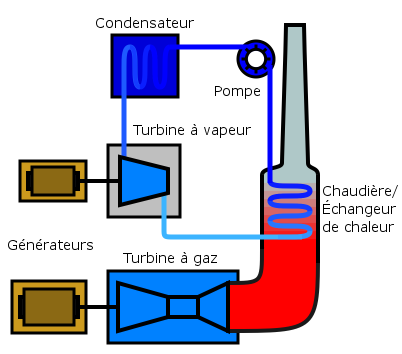
\includegraphics{figures/cycleTGCAV}	
	\caption{Exemple d'une installation à cycle combiné\label{fig:cycleTGCAV}}
\end{figure}

\subsection{Dérivez l'expression du rendement global $\eta_\text{TGCAV}$ d'un cycle combiné en fonction des températures des sommets du cycle.}
Pour obtenir le maximum de travail moteur des gaz d'échappement, on peut imaginer de les détendre de façon adiabatique et sans travaux dissipatifs de leur état initial 4 à un état final 5 d'entropie $S_4 = S_5$ et de température $T_5=T_1$, la pression $p_5$ étant dès lors bien inférieure à celle $p_1$ (voir diagramme $(T,S)$ figure \ref{fig:TScycleTGCAV}). Cette détente idéale produirait un travail moteur
\begin{equation} W_{mD} = H_4-H_1 \end{equation}
Afin de pouvoir rejeter dans l'atmosphère le fluide ainsi détendu, il faudrait alors le comprimer de $p_5$ à $p_1$, et consentir pour cela la consommation d'un travail moteur dont le miminum correspond à une compression isotherme utilisant l'atmosphère de température $T_1$ comme source froide. Le travail de compression aurait alors pour valeur 
\begin{equation} W_{mC} = T_1(S_4-S_1) \end{equation}
Ceci montre que l'exergie est bien le travail moteur maximum récupérable sur l'énergie disponibles des gaz d'échappement. Le rendement de conversion en travail de l'enthalpie sensible de ces gaz a donc pour valeur :
\begin{align} \eta_{CAV} &= \frac{W_{mD}-W_{mC}}{W_{mD}} \\ &= \frac{H_4-H_1-T_1(S_4-S_1)}{H_4-H_1} \\ &= \frac{c_p(T_4-T_1) - T_1c_p\ln\left(\frac{T_4}{T_1}\right)}{c_p(T_4-T_1)} \\ &= 1 - \frac{T_1}{T_4-T_1}\ln\left(\frac{T_4}{T_1}\right) \end{align}
En introduisant l'expression \ref{eq:q4_3} du rendement thermique du cycle de la turbine à gaz dans l'expression \ref{eq:eta_TGCAV} du rendement global on obtient :
\begin{equation} \eta_{TGCAV} = 1 - \frac{T_4-T_1}{T_3-T_2} + \frac{T_4-T_1}{T_3-T_2}\left(1-\frac{T_1}{T_4-T_1}\ln\left(\frac{T_4}{T_1}\right)\right) \end{equation}
Soit finalement :
\begin{equation} \eta_{TGCAV} = 1-\frac{T_1}{T_3-T_2}\ln\left(\frac{T_4}{T_1}\right) \end{equation}
\begin{figure}[p]\centering
	\tikzsetnextfilename{TScycleTGCAV}
    \begin{tikzpicture}
        \begin{axis}[%
    		enlargelimits=true,
        	grid=none,
        	axis lines=left, xtick=\empty, ytick=\empty,
        	xmin = 0, xmax = 6,
        	ymin = -1, ymax = 6,
        	ylabel=$T$,
        	xlabel=$S$,
        	no markers,
        ]        	
        	%\addplot+[domain=1:1.5,fill,blue!30] { 0.1899*5.2647^x - 1 } \closedcycle;
        	%\addplot+[domain=1.5:5,fill,blue!30] { 1.5197*1.3161^x - 1 } \closedcycle;
        	%\addplot+[domain=5:5.5,fill,blue!30] { 87.1945*0.5645^x } \closedcycle;
        	%\addplot+[domain=1:5.5,fill,white] { 0.7071*1.4142^x - 1 } \closedcycle;
        	%\addplot[dashed,domain=0:1] (1,x);
        	%\addplot[dashed,domain=1:1.5] { 1.5197*1.3161^x - 1 };
        	\addplot[black!50,domain=0.5:5.5] { 1.5197*1.3161^x - 1 } node[pos=0.5,sloped,above]{$p=\constant$};
        	\addplot[black!50,domain=0.5:6] { 0.7071*1.4142^x - 1 } node[pos=0.4,sloped,below]{$p=\constant$};
        	\addplot[domain=1.5:5] { 1.5197*1.3161^x - 1 };
        	\addplot[domain=5:5.5] { 87.1945*0.5645^x };
        	\addplot[domain=0:3.7568] (5.5,x);
        	\addplot[domain=1:5.5] {0};
        	%\addplot[domain=1:5.5] { 0.7071*1.4142^x - 1 };
        	\addplot[domain=1:1.5] { 0.1899*5.2647^x - 1 };
        	%\addplot[dashed,domain=3:5] (5,x);
        	
        	\draw (1,0) node{$\bullet$} node[below]{1};
        	%\draw (1,1) node{$\bullet$} node[above]{$2_S$};
        	\draw (1.5,1.2945) node{$\bullet$} node[above]{2};
        	%\draw (5,3) node{$\bullet$} node[below]{$4_S$};
        	\draw (5.5,3.7568) node{$\bullet$} node[right]{$4$};
        	\draw (5.5,0) node{$\bullet$} node[right]{$5$};
        	\draw (5,5) node{$\bullet$} node[above]{3};
    	\end{axis}
    \end{tikzpicture}
    \caption{Diagramme $(T,S)$ d'une installation à cycle combiné} 
    \label{fig:TScycleTGCAV}
\end{figure}

\subsection{Dérivez l'expression du rendement propulsif $\eta_P$ d'une turbine à gaz qui est utilisée en propulsion aérienne.}
Une turbine à gaz utilisée en propulsion aérienne crée la poussée $F$ destinée à compenser la traînée de l'avion et à lui conserver sa vitesse, par effet de réaction de l'air qui, s'approchant de l'avion à vitesse $c$ (dans un repère lié à l'avion), s'en éloigne à vitesse $c_s > c$ grâce à l'action du système propulsif. Pour un débit $\dot{m}$ passant dans le système propulsif, la relation fondamentale sur la conservation du flux de quantité de mouvement s'écrit :
\begin{equation} F = \dot{m}(c_s-c) \end{equation}
On définit la puissance propulsive par le produit de la poussée avec la vitesse de vol :
\begin{equation} P_p \triangleq Fc = \dot{m}(c_s-c)c \end{equation}
tandis que la puissance motrice dépensée résulte de la variation de l'énergie cinétique de l'air propulseur et a pour valeur :
\begin{equation} P_m = \dot{m}(\Delta K + W_f) \end{equation}
On exprime $W_f$ par une fraction de l'énergie cinétique de l'air qui transite dans le propulseur :
\begin{equation} W_f = (\xi-1)\frac{c_s^2}{2} \qquad \text{avec} \qquad \xi\geq 1 \end{equation}
et
\begin{equation} \Delta K = \frac{c_s^2-c^2}{2} \end{equation}
La puissance motrice s'écrit alors :
\begin{equation} P_m = \dot{m}\frac{\xi c_s^2-c^2}{2} \end{equation}
Le rendement propulsif a donc pour valeur :
\begin{equation} \eta_P = \frac{P_p}{P_m} = 2\frac{(c_s-c)c}{\xi c_s^2-c^2}  = 2\frac{\frac{c_s}{c}-1}{\xi\frac{c_s^2}{c^2}-1} \end{equation}
On voit que le rendement est fonction du rapport de vitesse et est optimum lorsque ce rapport a pour valeur :
\begin{equation} \frac{c_s}{c} = 1 + \sqrt{1-\frac{1}{\xi}} \end{equation}
À cette valeur, toujours inférieure à 2, correspond le rendement propulsif optimum de valeur :
\begin{equation} \eta_{P,max} = \frac{1}{\xi+\sqrt{\xi(\xi-1)}} \end{equation}

\subsection{Décrivez les avantages technologiques des turbines à gaz dans leur utilisation en propulsion aérienne et marine.}
Propulsion aérienne
\begin{itemize}
\item Le rapport puissance/masse de la turbine à gaz en fait le moteur idéalement compact pour la propulsion des avions.
\item La turbine à gaz répond à l'exigence d'une grande fiabilité mécanique liée à la relative simplicité de la maintenance.
\item La turbine à gaz dispose de grandes puissances unitaires pour voler vite et à haute altitude.
\item La diminution de $\rho_\text{air}$ ne constitue pas un handicap comparable à celui subi par les moteurs volumétriques.
\item L'abaissement de la température ambiante est très favorable au rendement par l'effet important qu'il a sur le rapport $Y = T_3/T_1$.
\end{itemize}

Propulsion marine 
\begin{itemize}
\item Le démarrage de l'ensemble rotorique est indépendant de l'actionnement du système propulsif.
\item La compacité d'une turbine à gaz
\end{itemize}

\section{Questions sur le chapitre ``Cycles thermodynamiques moteurs''}

\section{Questions sur le chapitre ``Cycles frigorifiques''}

\subsection{Dérivez l'expression du coefficient de performance (COP) pour un cycle inverse de Carnot.}
Le cycle inverse de Carnot est une référence théorique. Il s'agit d'un cycle $(T,S)$ rectangulaire (voir figure \ref{fig:TSCarnot}), comportant les transformation suivantes :
\begin{itemize}
\item Évaporation isotherme ($A\rightarrow B$) : $Q_I = T_I(S_B-S_A)$
\item Compression isentropique ($B\rightarrow C$) : $W_C = h_C-h_B$
\item Condensation isotherme ($C\rightarrow D$) : $|Q_{II}| = T_{II}(S_D-S_C) = T_{II}(S_B-S_A)$
\item Détente isentropique ($D\rightarrow A$) : $W_D = h_D - h_A$
\end{itemize}
Le coefficient de performance ou COP d'un cycle frigorifique est défini comme étant le rapport entre l'effet utile recherché et la dépense d'énergie :
\begin{equation} COP = \frac{Q_I}{W_C-W_D}\end{equation}
Or, $W_C-W_D$ vaut l'aire du rectangle $ABCD$, soit :
\begin{equation} W_C-W_D = (T_{II}-T_I)(S_B-S_A) \end{equation}
d'où :
\begin{equation} COP = \frac{T_I}{T_{II}-T_I} \end{equation}
\begin{figure}[p]\centering
	\tikzsetnextfilename{invCarnot}
    \begin{tikzpicture}
        \begin{axis}[%
    		axis lines=left, xtick=\empty, ytick=\empty,
        	grid=none,
        	xmin = 0, xmax = 8,
        	ymin = 0, ymax = 6,
        	ylabel=$T$,
        	xlabel=$S$,
        	no markers,
        	xticklabels={,,},yticklabels={,,},
        	extra x ticks={2,7},
		    extra x tick labels={$S_A$,$S_B$},
        	extra y ticks={2,5},
		    extra y tick labels={$T_I$,$T_{II}$}
        ]

        	\draw (2,2) node{$\bullet$} node[below right]{$A$} -- (2,5) node{$\bullet$} node[above]{$D$} -- (7,5) node{$\bullet$} node[above]{$C$} -- (7,2) node{$\bullet$} node[below right]{$B$} -- cycle;
        	\draw[dashed] (2,2) -- (2,0) node{$\circ$};
        	\draw[dashed] (2,2) -- (0,2) node{$\circ$};
        	\draw[dashed] (2,5) -- (0,5) node{$\circ$};
        	\draw[dashed] (7,2) -- (7,0) node{$\circ$};
        	\draw[<-] (4.5,3.5) +(80:1) arc(80:-260:1);
    	\end{axis}
    \end{tikzpicture}
    \caption{Diagramme $(T,S)$ du cycle inverse de Carnot}
    \label{fig:TSCarnot}
\end{figure}

\subsection{Dessinez le diagramme $log(p)-h$ d'un cycle frigorifique simple, à compression. Dérivez l'expression pour le coefficient de performance du cycle.}
La machine mettant en oeuvre un cycle frigorifique simple est représentée schématiquement à la figure \ref{fig:simplefrig}. Ce cycle comprend un compresseur, un condenseur, un détendeur et un évaporateur. On fait les hypothèses suivantes :
\begin{itemize}
\item la compression ($1 \rightarrow 2$) est isentropique;
\item la condensation ($2 \rightarrow 3$) et l'évaporation ($4 \rightarrow 1$) sont isobares; 
\item la détente ($3 \rightarrow 4$) est isenthalpique.
\end{itemize}
Le diagramme ($h$,$\ln p$) est disponible à la figure \ref{fig:diag_h_lnp}. Pour chacune des transformations on peut donc écrire :
\begin{itemize}
\item compression : $W_C = h_2-h_1$
\item condensation : $|Q_{II}| = h_2-h_3$
\item détente : $W_D = h_4-h_3 = 0$
\item évaporation : $Q_I = h_1-h_4$
\end{itemize}
Le coefficient de performance ou COP d'un cycle frigorifique est défini comme étant le rapport entre l'effet utile recherché et la dépense d'énergie :
\begin{equation} COP = \frac{Q_I}{W_C-W_D} = \frac{h_1-h_4}{h_2-h_1} \end{equation}

\begin{figure}[p]\centering
	\tikzsetnextfilename{schemaFrigoSimple}
	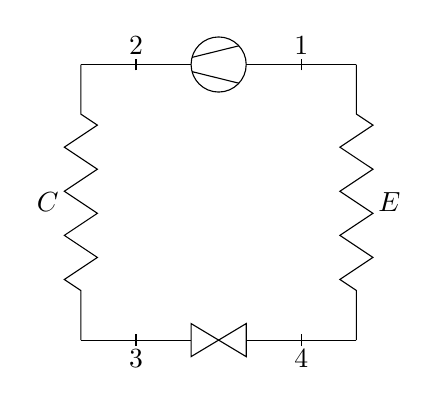
\begin{tikzpicture}[scale=0.7]
		\draw (0,0) -- (2,0) node[midway]{\rule{.4pt}{1ex}} node[midway,below]{3};
		\draw (2,-0.3) -- (2,0.3) -- (3,-0.3) -- (3,0.3) -- cycle;
		\draw (3,0) -- (5,0) node[midway]{\rule{.4pt}{1ex}} node[midway,below]{4};
		\draw (5.6,2.5) node{$E$};
		\draw (5,0) -- (5,0.9) -- (4.7,1.1) -- (5.3,1.5) -- (4.7,1.9) -- (5.3,2.3) -- (4.7,2.7) -- (5.3,3.1) -- (4.7,3.5) -- (5.3,3.9) -- (5,4.1) -- (5,5);
		\draw (2.02,5.13) -- (2.87,5.34);
		\draw (2.02,4.87) -- (2.87,4.66);
		\draw (5,5) -- (3,5) node[midway]{\rule{.4pt}{1ex}} node[midway,above]{1};
		\draw (2.5,5) circle (0.5);
		\draw (2,5) -- (0,5) node[midway]{\rule{.4pt}{1ex}} node[midway,above]{2};
		\draw (-0.6,2.5) node{$C$};
		\draw (0,0) -- (0,0.9) -- (-0.3,1.1) -- (0.3,1.5) -- (-0.3,1.9) -- (0.3,2.3) -- (-0.3,2.7) -- (0.3,3.1) -- (-0.3,3.5) -- (0.3,3.9) -- (0,4.1) -- (0,5);
	\end{tikzpicture}
	\caption{Schéma d'un cycle frigorifique simple}
	\label{fig:simplefrig}
\end{figure}

\begin{figure}[p]\centering
	\tikzsetnextfilename{diagramme_lnp_h}
    \begin{tikzpicture}
        \begin{axis}[
        	enlargelimits=true,
        	grid=major,
        	ymode=log,
        	axis lines=left, xtick=\empty, ytick=\empty,
        	xmin=0,xmax=3500,
        	ylabel=$\ln p$,
        	xlabel=$h$,
		]
			\addplot[black] table[col sep=comma,x index = {1}, y index = {0}] {data/lnp-h.csv};
			\addplot[black] table[col sep=comma,x index = {2}, y index = {0}] {data/lnp-h.csv};
			\draw[thick,red] (3300,1) node{$\bullet$} node[above right]{2} -- (762.5,1) node{$\bullet$} node[above left]{3} -- (762.5,0.01) node{$\bullet$} node[below left]{4} -- (2583.9,0.01) node{$\bullet$} node[below right]{1} to[bend left=-10] cycle;
        \end{axis}
    \end{tikzpicture}
    \caption{Diagramme ($h$,$\ln p$) d'un cycle frigorifique simple}
    \label{fig:diag_h_lnp}
\end{figure}

\subsection{Pourquoi faut-il choisir un fluide frigorigène dont la chaleur massique de la vapeur soit la plus faible possible ?}
Il en va de l'efficacité du cycle frigorifique. Le COP sera d'autant plus élevé que pour $Q_I$ fixé, on aura $W$ faible. Or :
\begin{equation} W = h_2-h_1 = c_PT_1\left[\left(\frac{p_2}{p_1}\right)^{\frac{k-1}{k}}-1\right] \end{equation}
et le rapport de compression $p_2/p_1$ est à peu près indépendant du fluide frigorigène choisi. En conséquence, il faudra choisir un fluide dont le $c_p$ soit la plus faible possible. 

\subsection{Donnez 5 critères technologiques, opérationnels et économiques de choix d'un fluide frigorigène.}
\begin{description}
\item[Coût du compresseur] : le coût est directement lié au débit volumique de fluide frigorigène en $1$. Soit $\dot{P}$ le débit massique de fluide frigorigène, on trouve :
\begin{equation} COP = \frac{\dot{P}Q_I}{\dot{P}W} = \frac{\dot{P}Q_I}{\rho_1\dot{V}_1W} \end{equation} 
Un bon indice de coût est le débit volumique de fluide frigorigène rapporté à l'unité de puissance frigorifique utile, soit :
\begin{equation} \text{coût compresseur } \simeq \frac{\dot{V}_1}{\dot{P}Q_I} = \frac{1}{\rho_1(h_1-h_4)} \end{equation}
On cherche donc un fluide frigorigène avec un grand $\rho$ et donc avec un poids moléculaire élevé.
\item[Pression $p_2$] : le coût de construction de la machine sera évidemment d'autant plus réduit que $p_2$ est modéré.
\item[Pression $p_4=p_1$] : il est important que la pression inférieure du cycle demeure légèrement supérieure à la pression atmosphérique. Il est préférable d'avoir une fuite qu'une rentrée d'air qui obligerait une purge complète et difficile de l'installation.
\item[Viscosité] : elle doit être faible, pour réduire les pertes par frottement et améliorer le transfert de chaleur.
\item[Conductivité thermique] : elle doit être élevée pour réduire la résistance thermique dans la couche limite en contact avec la paroi.
\item[Vitesse du son] : elle doit être élevée afin de permettre des vitesses du fluide très élevée dans le compresseur rotatif (uniquement pour des installations de grandes dimensions.
\item[Compatibilité] : avec l'huile de lubrification du compressuer et avec les matériaux du circuit. Exemple : l'ammoniac est incompatible avec le cuivre.
\item[Stabilité chimique] : la stabilité chimique permet des températures élevées en sortie du compresseur et réduit la déterioration du fluide dans le temps.
\item[Prix du fluide] : pas besoin d'explications.
\end{description}

\subsection{Pourquoi et comment est-ce qu'on réalise le sous-refroidissement du fluide frigorigène au condenseur ?}
Il est impératif, pour le bon fonctionnement de la machine frigorifique que la condensation du fluide frigorigène soit complète. Soit le cycle frigorifique (1-2-3-4-1) avec condensation complète à la figure \ref{fig:sousrefroid}. Supposons que la condensation soit franchement incomplète pour se terminer en A par exemple, (1-2-A-B-1). Le COP sera considérablement réduit car, si le travail de compression $(h_2-h_1)$ reste identique, l'effet utile $(h_1-h_B)$ lui, aura diminué :
\begin{equation} COP_{12AB} < COP_{1234} \end{equation}
Pour veiller au bon achèvement de la condensation, on se résout à prolonger la condensation par un sous-refroidissement du liquide saturé jusqu'au point 5, dont la température est légèrement inférieure à la température de condensation. Dans ce cas, le sous-refroidissement peut être obtenu grâce au fluide extérieur de refroidissement, par un surdimensionnement de la surface d'échange au condenseur. Un sous-refroidissement plus important peut être obtenu par échange interne à l'aide d'un échangeur additionnel (voir question suivante). 

Il est important de noter qu'un refroidissement effectué de la première manière (surdimensionnement) n'est pas favorable du point de vue des performances thermodynamiques. Le cycle (1-2-5-6-1) a effectivement un meilleur COP que le cycle (1-2-3-4-1), mais les températures de saturation au condenseur ne sont pas les mêmes. Si on compare le COP du cycle (1-2-5-6-1) avec celui du cycle (1-2'-5'-6-1) qui atteint la même température de saturation au condenseur, on observe :
\begin{equation} COP_{1256} < COP_{12'5'6} \end{equation}  
La pratique d'un sous-refroidissement, bien que nécessaire, est donc toujours défavorable du point de vue des performances thermodynamiques.

\begin{figure}[p]\centering
	\tikzsetnextfilename{sousRefroidissement}
    \begin{tikzpicture}
        \begin{axis}[
        	enlargelimits=true,
        	grid=major,
        	ymode=log,
        	axis lines=left, xtick=\empty, ytick=\empty,
        	xmin=0,xmax=3500,
        	ylabel=$\ln p$,
        	xlabel=$h$,
		]
			\addplot[black] table[col sep=comma,x index = {1}, y index = {0}] {data/lnp-h.csv};
			\addplot[black] table[col sep=comma,x index = {2}, y index = {0}] {data/lnp-h.csv};
			\draw[thick,red] (3300,1) node{$\bullet$} node[above right]{2} -- (762.5,1) node{$\bullet$} node[above]{3} -- (762.5,0.01) node{$\bullet$} node[below]{4} -- (2583.9,0.01) node{$\bullet$} node[below right]{1} to[bend left=-10] cycle;
			\draw[red] (1500,1) node{$\circ$} node[above]{$A$} -- (1500,0.01) node{$\circ$} node[below]{$B$};
			\draw[red] (762.5,1) -- (561.4,1) node{$\circ$} node[above]{$5$} -- (561.4,0.01) node{$\circ$} node[below]{$6$} -- (762.5,0.01);
			\draw[red] (762.5,1) -- (300,1) node{$\circ$} node[above]{$7$} -- (300,0.01) node{$\circ$} node[below]{$8$} -- (762.5,0.01);
			\draw[red] (561.4,0.3) node{$\circ$} node[left]{$5'$} -- (3180,0.3) node{$\circ$} node[right]{$2'$};
        \end{axis}
    \end{tikzpicture}
    \caption{Diagrammes ($h$,$\ln p$) de cycles frigorifiques simples (1-2-3-4-1) et (1-2'-5'-6-1), de cycles frigorifiques avec sous-refroidissement (1-2-5-6-1) et (1-2-7-8-1) et d'un cycle à condensation incomplète (1-2-A-B-1)}
    \label{fig:sousrefroid}
\end{figure}

\subsection{Expliquez pourquoi le coefficient de performance (COP) d'une installation frigorifique est indépendant d'un sous-refroidissement à l'aide d'un échangeur de chaleur additionnel.}
Le schéma d'une telle installation est disponible à la figure \ref{fig:frigoechangeur} et le diagramme $(h,\ln p)$ à la figure \ref{fig:sousrefroid}. La chaleur $\Delta Q$ échangée dans l'échangeur $E$ vaut :
\begin{equation} \Delta Q = h_3 - h_7 = h_4-h_8 \end{equation}
En fonctionnement normal (état 3 saturé), le coefficient de performance 
\begin{equation} COP = \frac{h_1-h_4}{h_2-h_1} \end{equation}
demeure indépendant de l'ampleur du sous-refroidissement grâce à l'égalité des longueurs des segments 73 et 84 et est égal à celui du cycle de référence (1-2-3-4-1).

\begin{figure}[p]\centering
	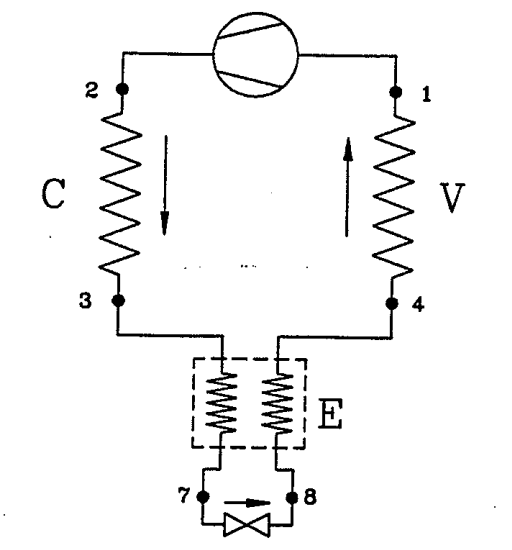
\includegraphics[height=7cm]{figures/frigoechangeur}
	\caption{Installation frigorifique à sous-refroidissement par échangeur de chaleur additionnel}
	\label{fig:frigoechangeur}
\end{figure}

\subsection{Quel est l'état désirable du fluide frigorigène à l'entrée du compresseur d'une installation frigorifique ? Comment peut-on contrôler cet état ?}
La présence de gouttelettes de liquide à l'aspiration du compresseur dégrade significativement son rendement. Un titre inférieur à 1 à l'entrée du compresseur est donc à éviter. À l'opposé, une surchauffe initiale accroît le travail moteur et dégrade donc le COP. 

Le choix le plus favorable est donc l'état saturé.

Pour les grosses installations, la configuration de la figure \ref{fig:grosfrigo} permet d'atteindre simplement le contrôle de cet état, par l'adjonction d'un séparateur $S$ à la sortie de l'évaporateur. On a également ajouté un dispositif optionnel $A$ qui, par effet d'éjection à la sortie du détendeur, permet d'intensifier la circulation naturelle dans l'évaporateur.

Pour les petites installations on adopte la disposition représentée à la figure \ref{fig:petitfrigo} : deux comparateurs de températures $CT1$ et $CT2$ permettent de vérifier en permanence, par l'existence de petits écarts de température, que l'évaporation et la condensation sont bien complètes. 

\begin{figure}[p]\centering
	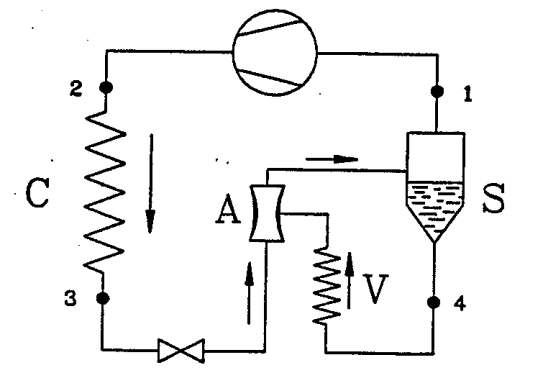
\includegraphics[height=5cm]{figures/grosfrigo}
	\caption{Installation frigorifique avec séparateur}
	\label{fig:grosfrigo}
\end{figure}
\begin{figure}[p]\centering
	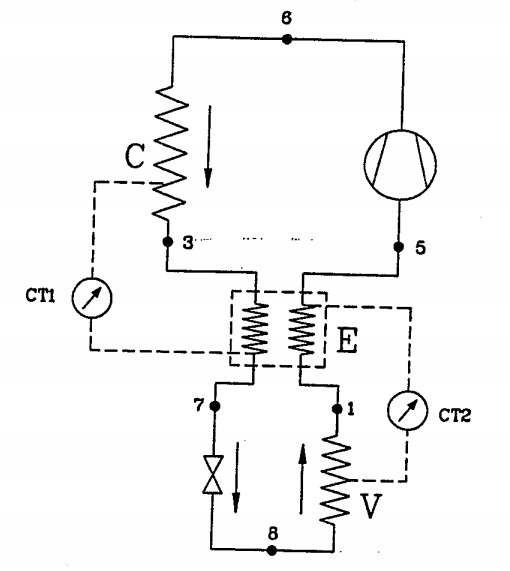
\includegraphics[height=7cm]{figures/petitfrigo}
	\caption{Installation frigorifique avec comparateurs de températures}
	\label{fig:petitfrigo}
\end{figure}

\subsection{Dérivez l'expression du coefficient de performance (COP) pour une pompe à chaleur.}
Une pompe à chaleur est constituée des mêmes organes qu'une machine frigorifique, mais son but est différent : son effet utile sera la production de chaleur au condenseur $C$ par prélèvement de chaleur à l'ambiance au moyen de l'évaporateur $V$ (voir figure \ref{fig:simplefrig} et \ref{fig:diag_h_lnp}).
L'effet utile est donc :
\begin{equation} |Q_{II}| h_2-h_3 \end{equation}
Le travail de compression reste le même que pour une installation frigorifique :
\begin{equation} W = h_2-h_1 \end{equation}
On a donc le coefficient de performance 
\begin{equation} COP = \frac{|Q_{II}|}{W} = \frac{h_2-h_3}{h_2-h_1} \end{equation}
Comme on a, par bilan d'énergie :
\begin{equation} Q_I + W = |Q_{II}| \end{equation}
On peut encore écrire :
\begin{equation} COP = 1 + \frac{Q_I}{W} \end{equation}



\end{document}
